\graphicspath{{sections/02_GCP_HOLO_Optimization/}}

\chapter{GCP-HOLO: Generating High-Order Linkage Graphs for Path Synthesis}\label{sec:gcpholo}
One degree of freedom (1DOF) linkages are persistent in mechanical systems. However, designing linkages to follow a desired path, known as path synthesis, is challenging due to non-linearities, combinatorial nature, and strict geometric constraints. Current state-of-the-art algorithms cannot scale well to linkages with higher-order linkage graphs, which are required to satisfy more complicated paths for new mechanical systems, such as hopping and flying robots. One reason for this is that state-of-the-art algorithms spend the majority of the time exploring constraint-violating designs. This work uses an Assur group 0DOF linkage as a graph grammar rule to modify both linkage graph and spatial parameters, ensuring all designs are valid 1DOF linkages. Using this graph grammar, this paper formulates linkage path synthesis as a tree search and uses a Deep Reinforcement Learning (DRL) agent to search the space of kinematically feasible planar 1DOF linkages. This paper introduces a method using a Graph Convolution Policy for High-Order Linkage Graph Optimization called GCP-HOLO. An any-time algorithm, GCP-HOLO outputs linkages with 1-8 loops (4-16 bars) efficiently. When comparing the GCP-HOLO formulation to a recent state-of-the-art paper that solves a Mixed Integer Conic Program, GCP-HOLO generates sets of solutions of varying linkage complexities to 8 test trajectories in a quarter of the time. Extending GCP-HOLO with a global node optimization, such as Covariance Matrix Adaptation Evolutionary Strategy, the results quickly converge to finding better solutions for 4/8 tests, with the whole pipeline capable of a 13X speed increase. 

\section{Introduction}
In the long history of the path synthesis problem, there still lacks a scalable method for simultaneous graph and geometric parameter design for path synthesis of high-order linkage graphs. This paper defines a high-order linkage graph as having 3 or more loops or greater or equal to an 8-bar linkage. A solution for this problem can help engineers explore new applications for linkages in designing mechanical systems. Linkages consistently have resurgences in the design of mechanical systems due to their ability to transform circular motion into any arbitrary path and improve the mechanical advantage of the end effector, such as the force and torque advantages. Recently, with stronger computational tools \cite{plecnik_computational_2016}, the design of more complex linkages advanced areas in modern robot designs \cite{ramezani_bat_2016, FestoUSA2018BionicFlyingFox, plecnik_design_2017}.  The 8-bar linkage design reduced the number of actuators used on the robot enabling highly dynamic behavior with overall lower weight and cost \cite{ramezani_bat_2016}, \cite{plecnik_design_2017}. Current systems still primarily focus on pure geometric optimization, which requires expert knowledge from the end-user, such as which linkage graphs will lend themselves to the desired trajectory. This work seeks to reduce the expertise needed of the end-user in solving path synthesis by introducing a method called GCP-HOLO (Graph Convolution Policy for High-Order Linkage Graph Optimization) which: 
\begin{enumerate}
    \item Explores both linkage graph and linkage geometry simultaneously;
    \item Provides sets of solutions with varying linkage graphs topologies rather than a point solution; 
    \item Can be augmented with other design constraints specific to the desired task.
\end{enumerate}
The problem of linkage design is challenging due to the mixed discrete and continuous design variables, non-linearities, combinatorial nature, and strict geometric constraints. This paper focuses on linkages defined by rigid bars connected by revolute joints. The configuration of bars and joints defines the linkage graph, and the location of the revolute joints or bar lengths defines the linkage geometry. The linkage graph configuration problem is a combinatorial discrete number problem with a long history of research related to the generation of unique configurations \cite{mruthyunjaya_kinematic_2003}. A notable solution to this problem was by Tuttle, who found all possible 1DOF mechanisms with up to 1–6 loops (4–12 bars) to be 4.3×106 configurations \cite{tuttle_generation_1996}. The linkage geometry problem is a continuous problem and has an equally long history of investigation. A pivotal contribution in this area was from Freudenstein, who created an analytical approach to solving the path synthesis problem for a one-loop (four-bar) linkage \cite{FerdinandFreudenstein1955}. It may be surprising that the progress in solving the path synthesis problem for higher-order linkage graphs is still very much unsolved. Recent works like  \cite{plecnik_designing_2020} found the 1.5×106 solutions to a two-loop (six-bar) linkage graph for a path synthesis problem. This paper considers three-loop (eight-bar) or greater linkages as high-order linkage graphs because there are no analytical approaches to solving the path synthesis problem. A few works, such as \cite{lipson_evolutionary_2008, vermeer_kinematic_2018, pan_joint_2022}, have attempted to solve the path synthesis problem by combining the linkage graph and geometry. These methods greatly support the end-user, who may not be an expert in mechanism design. The linkage designs for all these problems must satisfy the 1DOF constraint and the strict physical constraints of the rigid bar connections defined by the revolute joints.

This paper provides an automated method to address the three goals defined prior. This paper presents a fixed homogeneous action space to iteratively grow a base linkage using the Assur group RRR 0DOF kinematic chain \cite{Assur1913InvestigationII.}. The problem is formulated as a tree search where a reinforcement learning (RL) agent is trained to learn a search heuristic to efficiently find designs that minimize the coupler trajectory to the goal. The search agent explores various depths of the graph to consider different linkage topologies to present as a solution set. The paper compares GCP-HOLO to a recent work that attempts to solve a similar problem using a mixed integer conic program (MICP) formulation. The paper shows an example of an application of a linkage system with secondary design constraints by applying the method to designing a linkage for a walking system based on the TrotBot footpath. Finally, a deeper evaluation of reinforcement learning variants’ performance is considered. This test compares the GCP-HOLO with on-policy updates, GCP-HOLO with off-policy, and a baseline random search. The main contributions of this work are as follows:
\begin{enumerate} 
    \item A tree search formulation of linkage path synthesis problem with RL search agent;
    \item Linkage latent state representation using graph convolution network (GCN);
    \item Fast linkage generation and simulation using 0DOF Assur group rule and symbolic kinematics;
    \item An OpenAI Gym environment for linkage design that can be used as a testbed for future RL algorithms.
\end{enumerate}

\section{Related Works}
\subsection{Fixed Linkage Graph Optimization}
Many approaches to the path synthesis problem fix the discrete linkage graph a priori and optimize only the continuous geometric parameters to minimize the distance to the desired coupler trajectory. A state-of-the-art method for path synthesis with high precision uses a dimensional synthesis method known as homotopy continuation \cite{plecnik_computational_2016}. That method converts the non-linear system of equations that define the linkage in the various key point positions into a high-order polynomial. The formulation is then converted into a root-finding problem whichis solved for the geometric parameters. That methodcan solve a path that consists of nine sample points for a four-bar linkage \cite{wampler_complete_1992} and up to 11sample points for a six-bar linkage \cite{plecnik_design_2016}. The maximum number of sample points is determined by the number of unknown parameters defining the mechanism, for example, link lengths or joint positions. A key limitation of that method is the computational complexity and restriction on the number of precision points. Because of these scaling issues, no further extensions for higher-order linkages exist. That work solved the exact solutions that satisfy the precision points for low-order linkage graphs (four-bar and six-bar), where the problem this paper addresses is path synthesis for high-order linkage graphs ($\geq$ eight-bar). 

Stochastic optimization techniques, such as the covariance matrix adaptation evolutionary strategy (CMA-ES), are an approach that is capable of optimizing geometric parameters of higher-order linkages \cite{thomaszewski_computational_2014}. That method converges to reasonable solutions when the design parameters are bounded and strong initial solutions are provided. That method can be computationally expensive as most designs the method considers are kinematically invalid due to the strict geometric constraints. CMA-ES also fails when the optimization is unbounded, as many solutions tend towards infinity or propose unrealistic design parameters. GCP-HOLO can be extended using CMA-ES to improve the solutions through small changes to the joint locations. Section 4.1 shows an example of GCP-HOLO’s solutions improved with CMA-ES. 

The linkage kinematics can be described as closed-form equations for a class of linkages proposed by  \cite{bacher_linkedit_2015}, known as simple kinematic loops. Bächer et al. introduced a gradient-based method to update the continuous parameters in a real-time interactive system \cite{bacher_linkedit_2015}. That work showed that gradient descent is well suited when exploring the spatial parameters of a single linkage graph where a designer can influence different aspects of the linkage, such as scaling, specific node trajectories, or path constraints. That gradient-based approach quickly settles in a local minimum and only provides point-based solutions. That method could also be used to improve the final designs of GCP-HOLO, but since it natively does not consider the linkage graph variants, that work is not considered further in this paper. These fixed linkage graph approaches to path synthesis designs cannot simply be extended by iterating over all linkage graphs as the number of variations grows exponentially, with over 4.5×106 linkage graphs for linkages with less than 6 loops or 14 bars \cite{tuttle_generation_1996}.

\subsection{Simultaneous Linkage Design Optimization}
Recent work by Pan et al. \cite{pan_joint_2022} represents the problem as a MICP and solves for the optimal solution using a branch and bound method. That work showed significant progress in solving the planar path synthesis where both linkage graph and geometric parameters are solved simultaneously. However, some shortcomings are that the method cannot guarantee that intermediate designs are feasible, which requires the method to converge before a solution can be considered. Another limitation is that the computational complexity grows exponentially as the approach considers designs with higher linkage graphs, more sample points, or finer discretization. Finally, the method only provides a point solution, which may not be preferred in design automation as there are many considerations in the design that might not be expressed in the objective function, such as manufacturability and assembly. In this work, GCP-HOLO is an anytime algorithm that generates only kinematically feasible linkages addressing the intermediate design feasibility. GCP-HOLO also suffers from computational complexity but to a much lesser extent since invalid designs are prohibited from the formulation of the grammar rule. Finally, GCP-HOLO outputs a set of linkage designs of varying linkage topologies rather than a point solution. While MICP has some optimality guarantees, the planar path synthesis problem contains many local minima with objectives close to the optimal solution, as shown in the results in this paper. Therefore, this work can find several strong solutions in significantly less time, lending itself advantageously in certain situations. That work is compared to the current method in Sec. 4.1 as it most similarly addresses a comparable problem. 

Zhao et al. \cite{zhao_planar_2016} provided a mixed exact and approximate motion realization method that finds the optimal planar dyad chain. The planar dyad chain can then be converted into four-bar linkage solutions. Their approach converts the desired trajectory through kinematic mapping to a higher dimensional representation, the Image Space, that enables them to solve a least square fitting problem. The solution parameters from the least squares fitting are correlated to the different planar dyad types (RR, PR, RP). The advantage of this approach is that the solution found can have up to four precision poses and an arbitrary number of inexact poses. One limitation of this approach is that the desired trajectory must be satisfied by a planar dyad, which could be hard to determine a priori if the dyad is well suited for the path. 

Lipson proposed a genetic algorithm for linkage synthesis that simultaneously acts on the design’s linkage graph and spatial parameters with graph grammars \cite{lipson_evolutionary_2008}. Graph grammars are a set of pre-specified rules that modifies the current state by either adding to the graph, removing parts of the graph, or augmenting the graph structure. The graph grammars that Lipson defined were applied to the rigid bars of the linkage, which requires the forward kinematics (FK) of the new design to be fully re-evaluated. Since the FK must be evaluated thousands of times in genetic algorithms and RL, an efficient method for computing the FK must be considered. This paper defines the grammar rule on the nodes to address this issue, which only requires the added component’sFK to be evaluated using the symbolic kinematics method. Another limitation of Lipson’s grammar rules is the lack of constraints on the new joint’s initial location, which can lead to the evaluation of manykinematically degenerate designs. This paper uses a simplif ied constraint satisfaction criteria to evaluate the validity of new joint locations quickly. Finally, this paper extends the applications shown in Lipson, which only explored linkage design for a straight-line synthesis problem. This paper is applied to the more general path synthesis problem.

Vermeer et al. \cite{vermeer_kinematic_2018} trained a deep RL agent to learn a policy to apply Lipson’s grammar rules. To use Lipson’s grammar in their RL framework, Vermeer et al. introduced a spatial constraint such that the new node added forms an isosceles triangle. This constraint converts the graph grammar to a fixed action space more suitable for RL. However, that constraint impaired their method’s performance in generating designs and failed to achieve comparable results to Lipson’s method. That constraint also fails to guarantee a valid design since the isosceles triangle only satisfies the linkage constraints in the first time-step and not the whole trajectory. To address these limitations, this work replaces their spatial constraint with a set of scaffold nodes—a set of potential initial joint locations. This achieves a suitable action space for the RL agent with relaxed design limitations. This paper also uses a simplified constraint satisfaction criteria that check the validity of the node positions through the whole trajectory and not the initial time-step to prevent the evaluation of constraint-violating designs. Vermeer et al. defined the state of the linkage using hand-crafted features. This is inferior to learned feature representation using deep learning \cite{nanni_handcrafted_2017}. Therefore, in this work, a graph embedding network is used to learn the latent features of the current design state.

GCP-HOLO improves and differs from the prior works by defining a graph grammar rule that does not affect prior revolute joints’ trajectories and therefore avoids re-evaluation of the full forward kinematics. GCP-HOLO introduces scaffold nodes to extend the linkage configuration with a simplified constraint satisfaction criteria that quickly identifies the set of valid states, ensuring an anytime algorithm that generates valid 1DOF linkages. GCP-HOLO converts the graph representation of the linkage into a vector through a learned mapping. Finally, GCP-HOLO trains an RL agent to learn a search direction that improves the generation of linkages to satisfy the path synthesis problem.

\subsection{Reinforcement Learning in Design}
GCP-HOLO was inspired by several recent works that used deep RL agents to find solutions for design automation problems. Similar methods to GCP-HOLO have been used in solving problems related to truss design \cite{raina_learning_2019}, molecules design \cite{you_graph_2018}, and robot design \cite{whitman_modular_2020, zhao_robogrammar_2020}. RL-based methods provide a sequential design approach that Raina et al. [19] stated is comparable to human engineering design. You et al. argued that deep RL methods are more robust than other machine learning-based generative methods for designing physical systems, as RL can ensure that all physical constraints of the design problem are satisfied \cite{you_graph_2018}. GCP-HOLO uses reinforcement learning rather than other tree search methods, as it has been shown in \cite{you_graph_2018, whitman_modular_2020, zhao_robogrammar_2020, raina_goal-directed_2021} to outperform search algorithms, such as Monte Carlo Tree Search and best-first search.

Several areas differentiate the RL pipelines in each of those works. First, the state representation of the design can vary. Trusses, molecules, and robot configurations are all fixed systems, whereas linkages are time-varying periodic systems. For example, in Raina et al. \cite{raina_learning_2019}, images of trusses are used to evaluate the current state of the design. In  \cite{you_graph_2018, whitman_modular_2020, zhao_robogrammar_2020}, the design state of the molecule and robots are represented as a graph. This work uses a graph representation to represent the time-varying linkage. Second is the agent design itself; Whitman et al. \cite{whitman_modular_2020}, and Zhao et al. \cite{zhao_robogrammar_2020}, proposed deep Q-network (DQN), an off-policy network, and You et al. \cite{you_graph_2018}, used proximal policy optimization (PPO), an on-policy algorithm. An on-policy RL algorithm updates the policy network directly responsible for selecting the action with the most recent data generated from the rollouts. An off-policy RL algorithm keeps track of a history of data generated from the rollouts and randomly samples from this buffer to update the network. This work explicitly compares the different policies’ performance for the linkage generation problem.

\begin{figure}
    \centering
    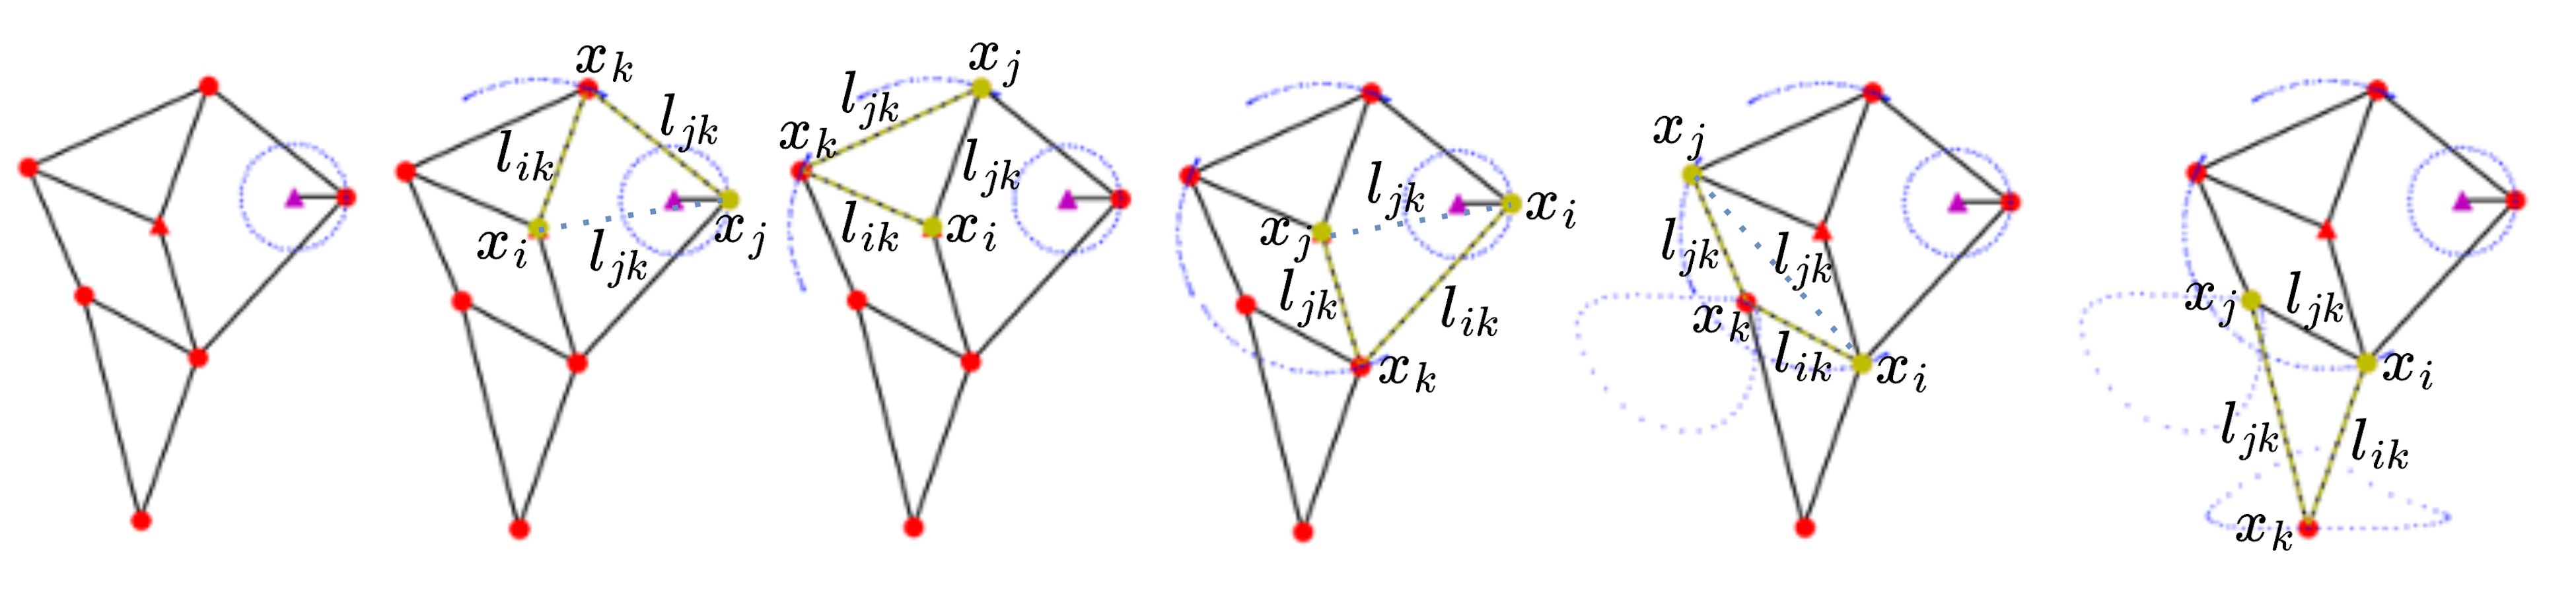
\includegraphics[width=\linewidth]{01_figure_Symbolic Kinematics_revision.png}
    \caption{Symbolic kinematic recursive FK process is shown on Jansen Linkage}
    \label{fig:symbolic_kinemtics}
\end{figure}

\section{Method}
Section \ref{sec:linkage-form} describes the class of linkages that this work considers and the simulation method to obtain the coupler trajectory. Section \ref{sec:gcp-holo} describes the GCP-HOLO algorithm, which includes Sec. \ref{sec:state-rep}, describing the linkage state representation as a graph and the GCN to learn the latent state representation. Section \ref{sec:action-rep} defines the action space from the graph grammar rule to explore linkage designs. Section \ref{sec:design-obj} shows the objective of the path synthesis problem and reward design used to train the reinforcement learning agent. Finally, Sec. \ref{sec:training} describes the different types of reinforcement learning algorithms that can be used and the training process for the method.

\subsection{Linkage Formulation}\label{sec:linkage-form}
The kinematic chains this work designs can be understood as 1DOF high-order planar linkage graphs with simple kinematic loops. This section provides a breakdown of each of those terms to better inform the reader. One degrees-of-freedom (1DOF) defines the number of input variables needed to define the linkage pose fully. The type of linkages this paper designs consists of a set of moveable and fixed revolute joints connected by a set of rigid links and a motor input. For the 1DOF system knowing the angle of the motor input is sufficient to know the position of the rest of the mechanism. A complete revolution of the motor generates periodic paths for each moveable revolute joint. Gruebler’s formula, shown in Eq. \eqref{eq:dof}, can be used to verify the degrees-of-freedom of the system:
\begin{equation}\label{eq:dof}
    DOF = 3(n-1)-2j
\end{equation}
where n is the total number of links, j is the total number of revolute joints.

In planar mechanisms, all the revolute joints and rigid bars exist in the XY-plane. This is useful for designing linkages in simulation and determining the trajectories of the revolute joints. This can cause conflicts when converting designs from simulation to reality as the manufacturability and linkage assembly aren’t considered.

The configuration of the revolute joints and rigid bar components describes the linkage graph. The rigid bars in the linkage create closed loop structures. The linkage community, rather than describing the systems by the loops refers to them as four-bar (one loop), six-bar (two loops), eight-bar (three loops), etc. This paper defines higher-order linkage graphs with linkages that have $\geq$3 active loops, this is because there are no analytical approaches to solving the path synthesis of linkages with $\geq$3 active loops. The Jansen linkage in Fig. \ref{fig:symbolic_kinemtics} is an example of a high-order linkage graph as it contains three loops \cite{Jansen1990Strandbeast}. This work uses the minimum cycle basis method to find the number of active loops that comprises the linkage graph \cite{kavitha_tildeom2n_2008}.

In our work, the forward kinematics must be evaluated hundreds of thousands if not millions of times. A recursive approach for solving the forward kinematics for closed loop systems provides faster evaluations than constraint-based methods as described in \cite{kecskemethy_symbolic_1997}. Bächer et al. \cite{bacher_linkedit_2015} described a recursive method, symbolic kinematics, to quickly evaluate the forward kinematics for a subset of linkage graphs made up of revolute joints. This method does not work for all linkage graphs but does span 7 out of the 11 planar 1DOF eight-bar linkage topologies described by Tsai and Mccarthy \cite{tsai_mechanism_2000}. Symbolic kinematics is also not currently suited for systems with prismatic joints, so prismatic joints are not considered in this work. Symbolic kinematics represents the linkage by its joint positions and distance constraints between connected revolute joints. The crank joint location is determined from the motor input angles, given by:
\begin{equation}
    x_{\text{crank}}(t) = R(\lambda \theta(t)) \cdot (x_{\text{crank}}(1) - x_{\text{motor}}) + x_{\text{motor}}, \quad \forall t \in [2, T]
\end{equation}
where $R(\cdot)$ is the 2x2 rotation matrix, $\lambda$ is the direction of the motor with $\lambda = \begin{cases}
    1, & \text{CCW}.\\
    -1, & \text{CW}.\end{cases}$ and $x(t)$ is the planar position of the joint at time $t$. This paper evenly spaces the set of discrete angles, $\theta(t)$, from 0 to $2\pi$ to generate the linkage trajectories, but any partial set of motor angles can be specified a priori. All other revolute joints, $x_k(t)$, can be found when two neighboring joint locations, $x_i(t)$ and $x_j(t)$, are known. This can be understood geometrically by finding the intersection of two circles centered at the known joints’ locations with radii equal to the fixed distances to the unknown joint, respectively. The complete expression for this algebraically can be seen in:
\begin{align}
    x_k(t) &= R(\lambda \phi(t)) \cdot \frac{l_{ik}}{l_{ij}(t)} (x_{j}(t) - x_{i}(t)) + x_{i}(t), \quad \forall t \in [2,T], \\
    \phi(t) &= \arccos\left(\frac{l_{ij}(t)^2 + l_{ik}^2 - l_{jk}^2}{2 l_{ij}(t) l_{ik}}\right)
\end{align}
where the fixed side lengths are defined as \( l_{ik} = \| x_i(1) - x_k(1) \| \) and \( l_{jk} = \| x_j(1) - x_k(1) \| \). The final variable side length is \( l_{ij}(t) = \| x_i(t) - x_j(t) \| \). From the two solutions, \( \lambda = \pm 1 \), the one that matches the given initial joint location \( x_k(1) \) is used, and the solution sign is maintained through all time-steps. The reader is referred to Refs.~\cite{pan_joint_2022,bacher_linkedit_2015} for a full description of symbolic kinematics. An example of the iterative process of symbolic kinematics on the Jansen linkage can be seen in Fig.~\ref{fig:symbolic_kinemtics}.


\begin{figure}
    \centering
    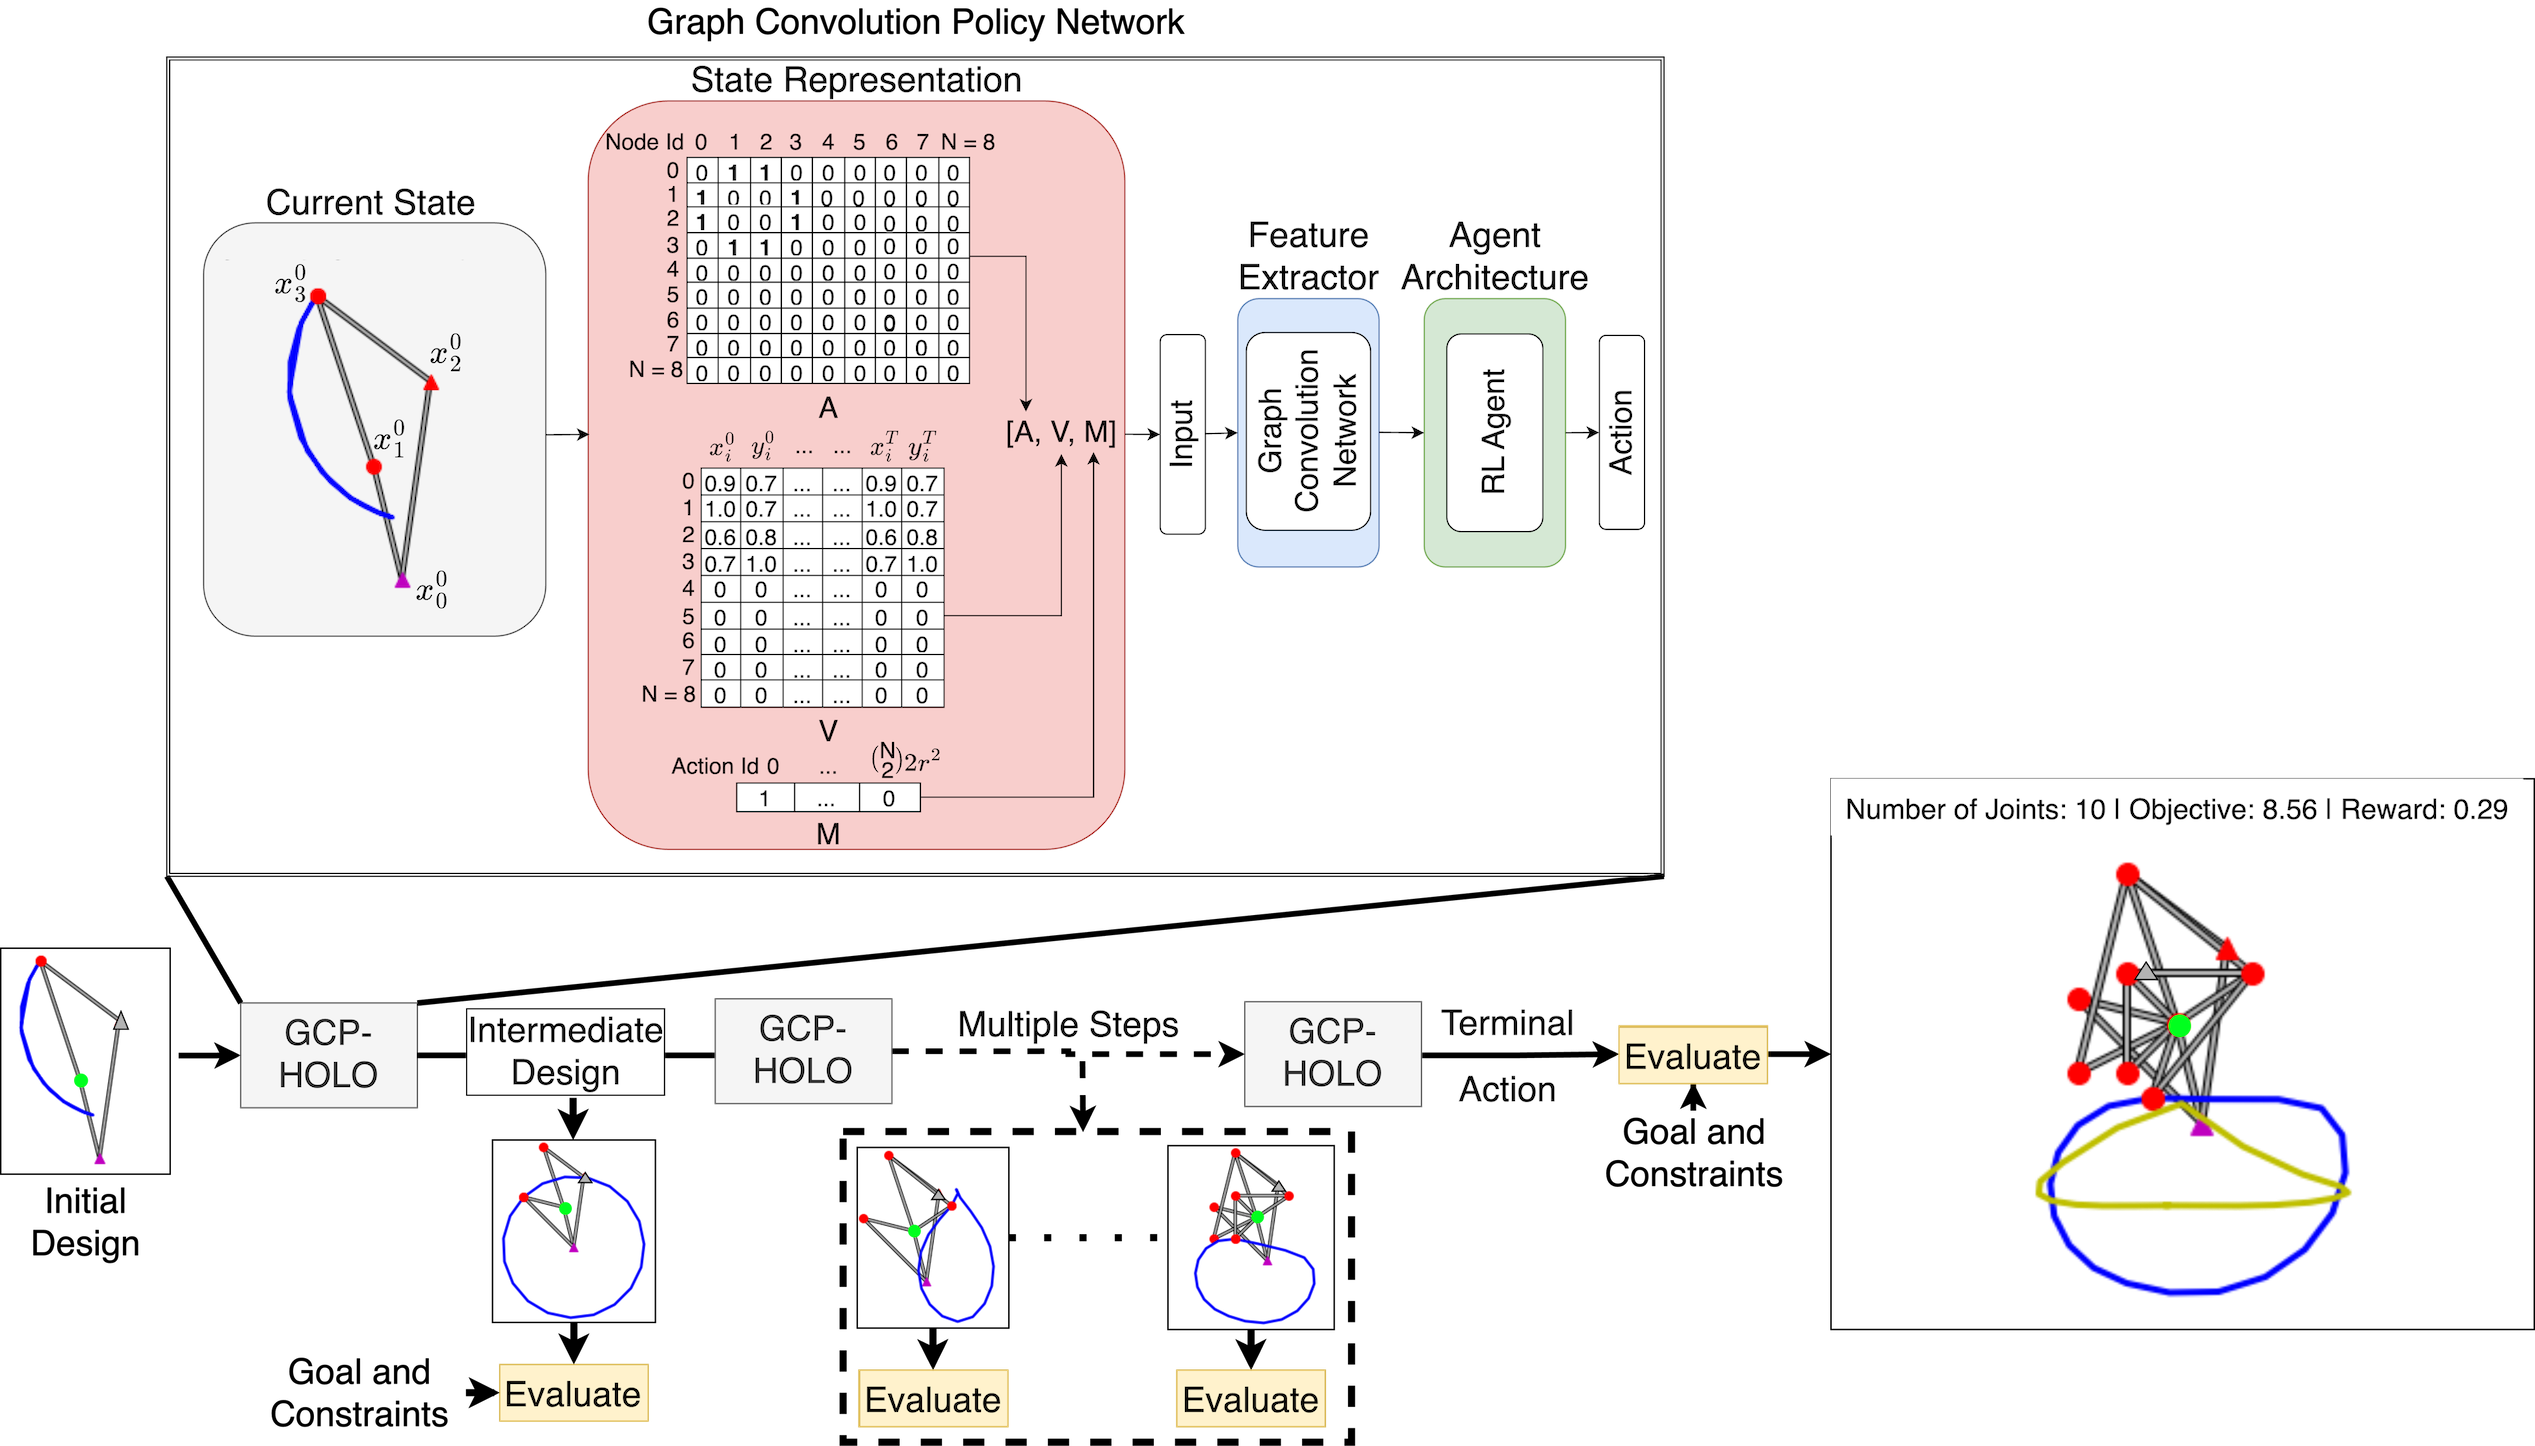
\includegraphics[width=\linewidth]{02_figure_block_diagram_revised.png}
    \caption{Block diagram of GCP-HOLO linkage design}
    \label{fig:gcp-holo_block}
\end{figure}

\subsection{GCP-HOLO}\label{sec:gcp-holo}
GCP-HOLO is a learning-based directed stochastic search algorithm for high-order linkage graphs to provide sets of solutions to the problem of path synthesis that is amenable to graphic processing unit (GPU) utilization for enhanced performance. A block diagram of the method can be seen in Fig. \ref{fig:gcp-holo_block}. This section breaks down the GCP-HOLO method in the following way. In Sec. \ref{sec:state-rep}, the state representation of the linkage as well as the GCN is described. In Sec. \ref{sec:action-rep}, the action space, as well as a simplified constraint satisfaction criteria to reduce the number of invalid actions, are explained. In Sec. \ref{sec:design-obj}, the reward design and path synthesis objective are defined. Finally, Sec. \ref{sec:training} shows the training and evaluation procedures for the reinforcement learning policy.

\subsubsection{State Representation}\label{sec:state-rep} In deviation from the standard graph representation of a linkage, this paper defines a linkage as a graph $G$, with nodes, $V$, representing the revolute joints, and the edges, $E$, representing the rigid bars. This deviation is because in the kinematic equations used, the linkage is described by the timevarying position of the revolute joints and distance constraints, rather than fixed reference frames on the rigid links. For the purposes of the graph neural network, the set of edges, $E$, are better described using an adjacency matrix $A$. The adjacency matrix is a binary symmetric matrix, where $A_{i,j}$ is one if the nodes $i$ and $j$ are connected and otherwise zero. This adjacency representation known as the linkage adjacency matrix in other historical works is most widely used \cite{mruthyunjaya_kinematic_2003}. The numeric labeling of the nodes must follow the hierarchy defined by Ref. \cite{bacher_linkedit_2015} such that higher number node indexes are dependent on lower number node indexes. This is always satisfied with the graph grammar rule in Figure~\ref{fig:assur_group}.

It is typical to map a system’s state representation into a vector in an RL pipeline using a feature extractor, for example, converting the linkage graph G to a vector equivalent. Learned feature extractors using neural networks outperform hand-crafted approaches. The feature extractor in GCP-HOLO is a GCN \cite{kipf_semi-supervised_2016} that maps the linkage graph previously described to a lower dimensional vector that encodes pertinent information about the graph. The GCN takes in the node features V along with the adjacency matrix A, which it uses as a convolutional filter, to linearly combine the connected node features. The convolution is followed by a fully connected layer that applies a non-linear activation function to the convolved features. The parameters of the GCN are updated using gradient descent throughout the training process. The GCN this work uses is the same architecture as Zhao et al. \cite{zhao_robogrammar_2020}, shown in Fig. \ref{fig:ppo-dqn}—further optimization on the feature extractor network architecture could provide additional performance improvements. Graph networks are permutation invariant and equivariant, meaning that node index permutations do not affect the output of the feature extractor \cite{maron_invariant_2019}. This is very useful for this problem because sets of actions applied in different orders can lead to the same linkage but different node index ordering. The mapping of these distinct linkage graphs from the graph network will be the same. The feature extractor and the agent are trained end-to-end, improving the learned mapping over time. A diagram of the RL pipeline is shown in Fig.~\ref{fig:gcp-holo_block}.

\subsubsection{Action Space}\label{sec:action-rep} The grammar rule in this work is defined such that previously evaluated revolute joint kinematics remain unchanged. By avoiding full forward kinematics (FK) evaluation at every step, the computation speed increased by 26\%. The left-hand side of the rule selects two nodes, \( i \) and \( j \), from the current linkage and attaches them to a new node \( k \) within the design space. The grammar rule is illustrated in Fig.~\ref{fig:assur_group}, where \( x_i(t) \) denotes the position of node \( i \) at time \( t = 1 \).

\begin{figure}
    \centering
    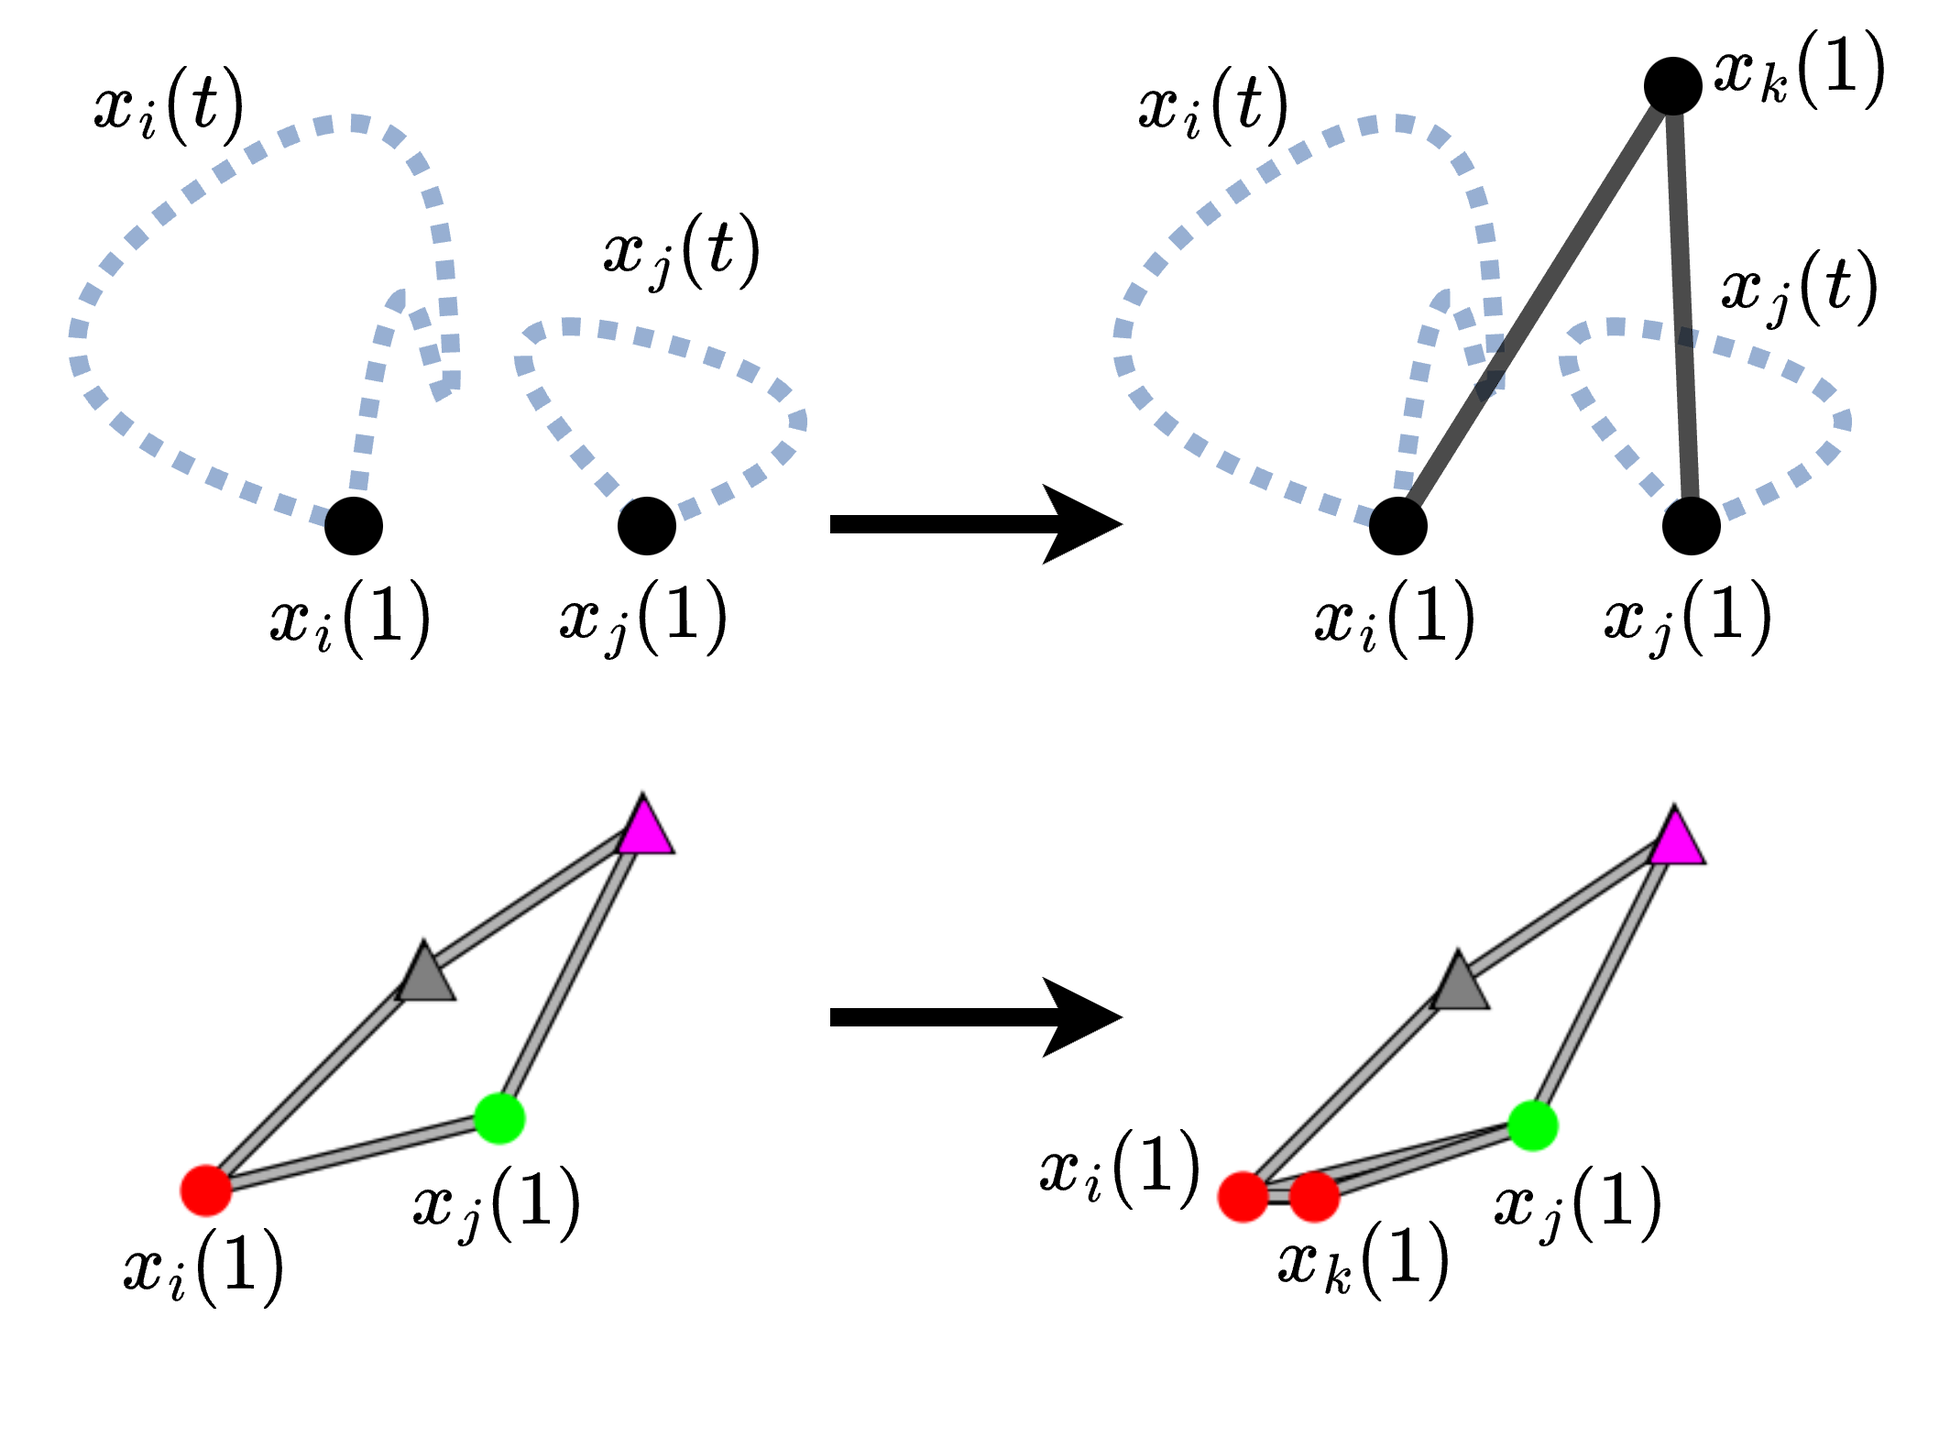
\includegraphics[width=0.65\linewidth]{03_figure_grammar_rule.png}
    \caption{0DOF Assur group graph grammar rule}
    \label{fig:assur_group}
\end{figure}
\begin{figure}
    \centering
    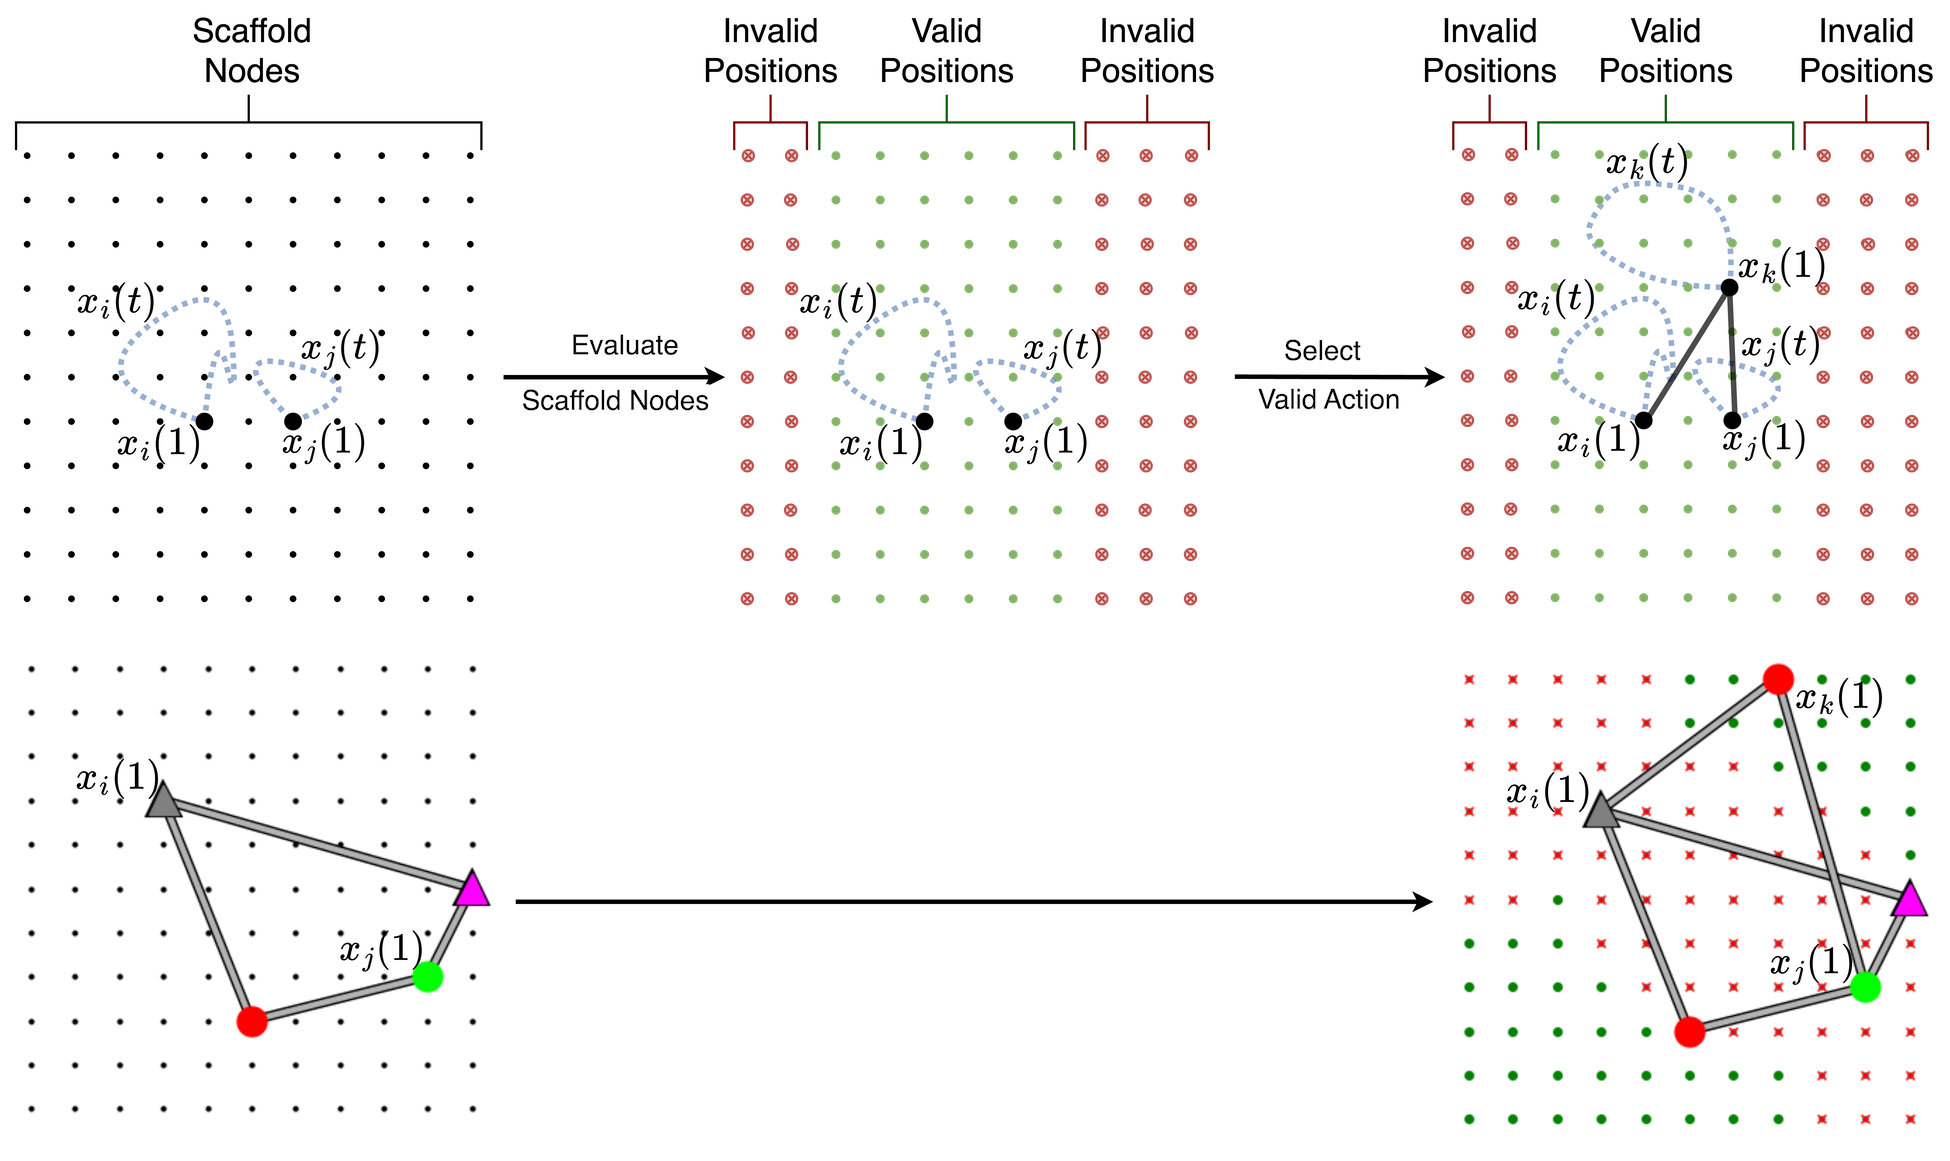
\includegraphics[width=\linewidth]{04_figure_scaffold_nodes.png}
    \caption{Graph grammar rule with scaffold nodes and simplified constraint satisfaction criteria}
    \label{fig:scaffold-nodes}
\end{figure}

To avoid constraint-violating positions for the new revolute joint, \( x_k(t) \), a simplified constraint satisfaction criterion is presented, as shown in Fig.~\ref{fig:scaffold-nodes}. First, a discrete set of positions, known as \textit{scaffold nodes}, is considered for \( x_k(1) \). Next, the fixed link lengths defined by each scaffold node, \( l_{ik} = \| x_i(1) - x_k(1) \| \) and \( l_{jk} = \| x_j(1) - x_k(1) \| \), along with the potentially varying length defined by the revolute joints, \( l_{ij}(t) = \| x_i(t) - x_j(t) \| \), are evaluated for triangle inequality conditions across all time steps. This check can be efficiently evaluated using vectorized programming and is described in Algorithm~\ref{alg:valid_scaffold}. While this method does not eliminate all invalid designs, it successfully prohibits the majority. In a small test of 1000 random rollouts, 81\% of the designs were kinematically invalid without this heuristic, whereas only 2\% were invalid when the heuristic was applied. This allows for the search algorithm to focus more on finding the coupler trajectory that best matches the desired goal, versus evaluating lots of invalid designs. To further prohibit all constraint-violating designs, such as cases with singularities, a description is provided at the end of Sec. \ref{sec:design-obj} when discussing the action acceptance criteria.

\begin{algorithm}[H]
\caption{Valid Scaffold Nodes}
\label{alg:valid_scaffold}
\begin{algorithmic}[1]
\Require $x_i$, $x_j$, $S$ \Comment{The trajectory of two revolute joints and the grid of scaffold node locations}
\State $l_{ij}(t) \gets \|x_i(t) - x_j(t)\| \quad \forall t \in [1, T]$ \Comment{Distance between nodes $i$, $j$ during revolution}
\State $l_{ik} \gets \|x_i(1) - S_k\| \quad \forall k \in [1, K]$ \Comment{Initial distance: node $i$ to scaffold $k$}
\State $l_{jk} \gets \|x_j(1) - S_k\| \quad \forall k \in [1, K]$ \Comment{Initial distance: node $j$ to scaffold $k$}
\Statex
\State $V_k = \texttt{all} \left( 
    \begin{aligned}
        & l_{ik} + l_{jk} > l_{ij}(t) \quad \forall t \in [1, T] \\
        \land & l_{ik} + l_{ij}(t) > l_{jk} \quad \forall t \in [1, T] \\
        \land & l_{ij}(t) + l_{jk} > l_{ik} \quad \forall t \in [1, T] 
    \end{aligned} \right)
    \quad \forall k \in [1, K]$
\State \Return $V$
\end{algorithmic}
\end{algorithm}

The total number of actions at any step in the design search is \( 2 {n\choose{2}}\cdot r^2 \), where \( n \) is the total number of nodes in the current state and \( r \) is the resolution of the discretized design space. Each action can be either an intermediate or a terminal action. The number of scaffold nodes is determined by a user-specified resolution \( r \) for both the \( x \)- and \( y \)-axes. As the resolution tends toward infinity, \( r \rightarrow \infty \), the discrete representation becomes equivalent to the continuous problem. However, higher resolution discretization increases computational cost and reduces runtime performance. The set of valid actions for all node pairs \( (i, j) \) is described in Algorithm~\ref{alg:valid_actions}. The valid actions for each set of node pairs are only computed once and can be cached for all future steps within an episode, as the valid actions for a given pair do not change when new nodes are added to the graph. Whereas most prior work spends the majority of time evaluating degenerate designs, Algorithm~\ref{alg:valid_scaffold} and Algorithm~\ref{alg:valid_actions} effectively prohibit the evaluation of most constraint-violating designs.

\begin{algorithm}[H]
\caption{Valid Actions}
\label{alg:valid_actions}
\begin{algorithmic}[1]
\Require $x_{1:n}$ \Comment{The trajectory of all revolute joints}
\State $mask \gets \emptyset$ \Comment{Initialize action mask}
\State $n \gets \textsc{NumberOfNodes}(x_{1:n})$ \Comment{Get current number of nodes}
\State $combs \gets \textsc{combinations}(n, 2)$ \Comment{Get all $i, j$ node pairs}
\For{$(i, j) \in combs$}
    \State $mask_{i,j,k} \gets \textsc{ValidScaffoldNodes}(x_i, x_j, S) \quad \forall k \in [1, K]$ 
    \Comment{Update mask with valid scaffold nodes}
\EndFor
\State \Return $mask$
\end{algorithmic}
\end{algorithm}

When the agent applies a terminal action, the final design can be pruned to only contain the revolute joints which are actively contributing to the coupler trajectory. This is done by recursively traversing from the coupler node to the root, keeping only the parent nodes that were used to solve the FKs for the coupler. All nodes that do not influence the coupler, are unnecessary and do not affect the kinematics of the coupler node. After pruning, the number of active loops that make up the linkage graph can be determined, and the reward of the linkage is determined. Figure \ref{fig:tree-search} shows a visualization of the sequential actions starting with a random valid root node and evaluating with respect to the Jansen footpath and Fig. \ref{fig:prune-linkage} shows a pruning from a terminal design.

\begin{figure}
    \centering
    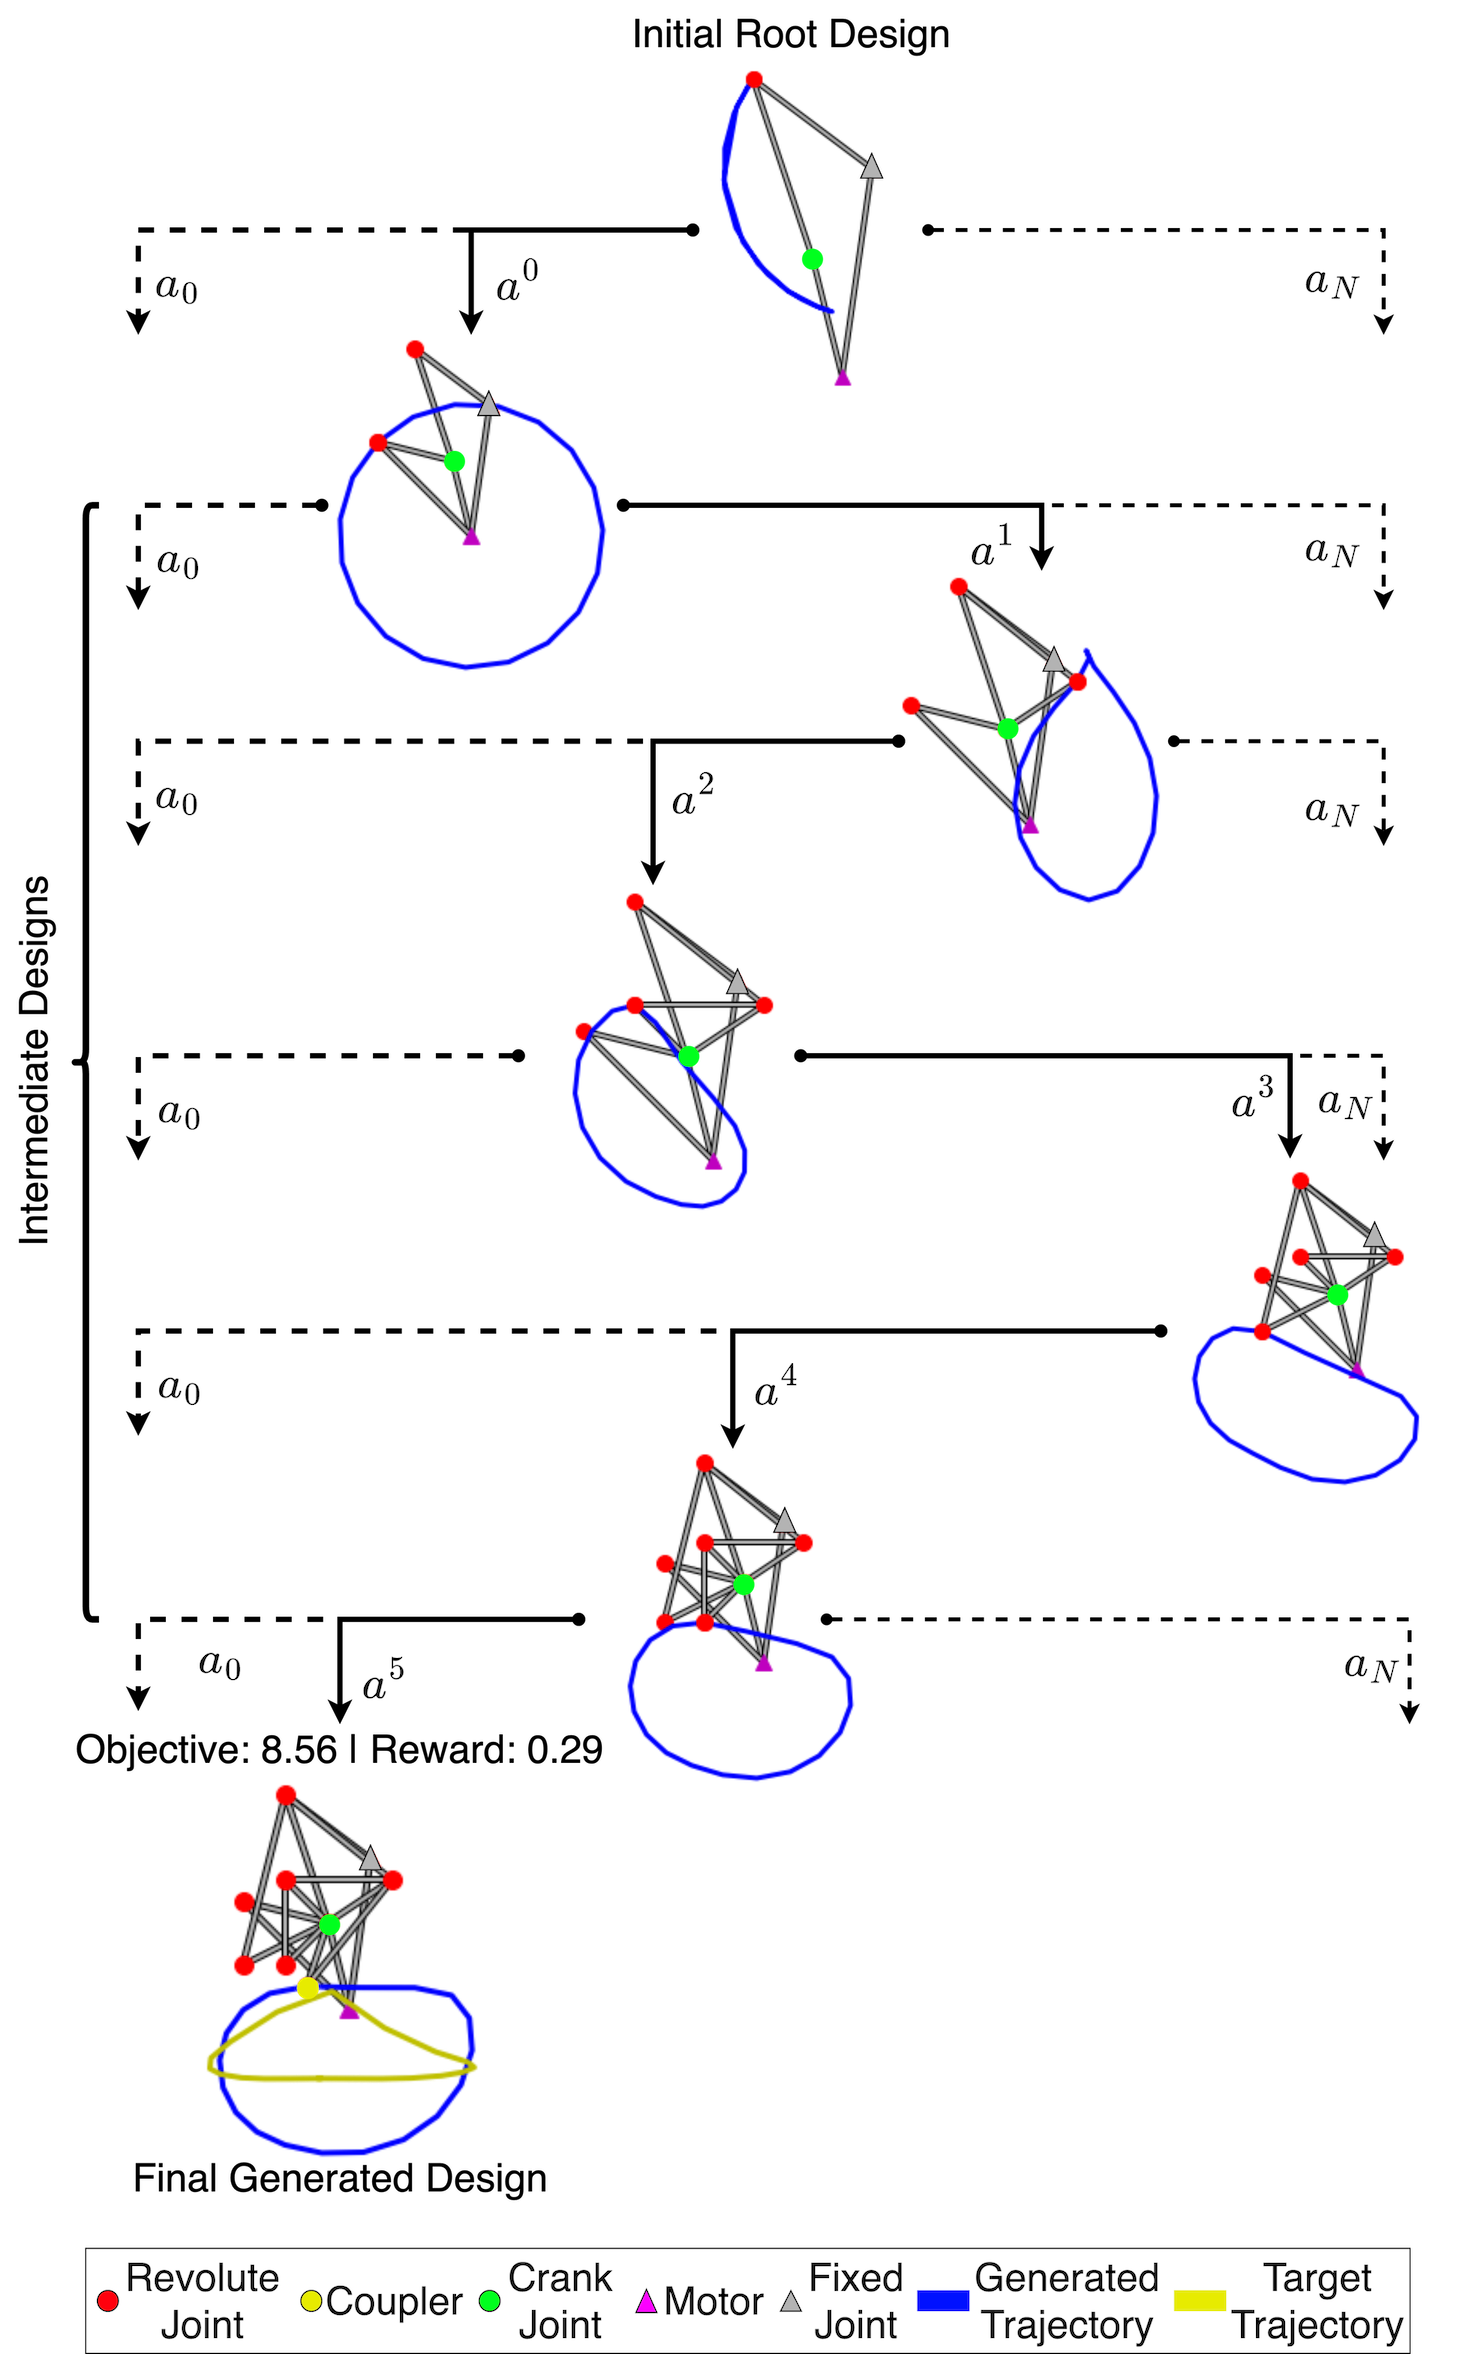
\includegraphics[height=0.9\textheight]{05_figure_graph_search.png}
    \caption{Linkage design as discrete tree search}
    \label{fig:tree-search}
\end{figure}

\begin{figure}
    \centering
    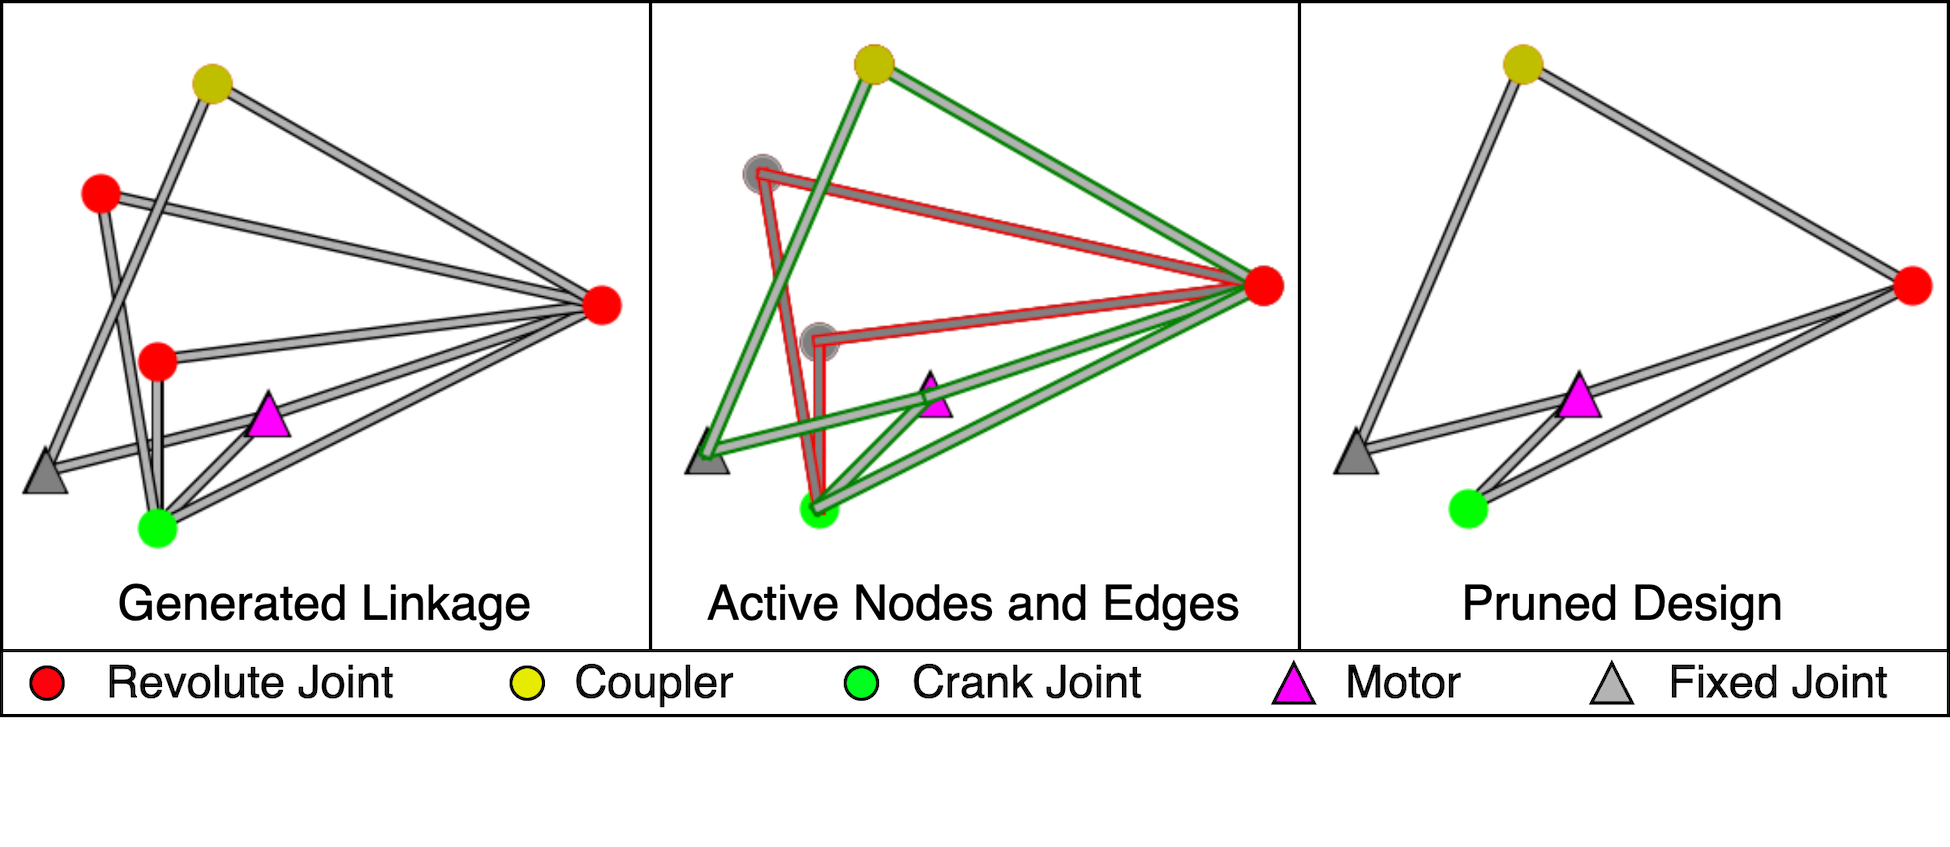
\includegraphics[width=0.9\linewidth]{06_figure_Prune_diagram.png}
    \caption{Pruning generated linkage of unused joints and edges}
    \label{fig:prune-linkage}
\end{figure}

\subsubsection{Design Objective}\label{sec:design-obj} The terminal node added to the linkage is known as the coupler node, $x_N$, and defines the trajectory that this paper seeks to optimize. To compare the coupler trajectory with the goal trajectory, \( x^*_N \), the average norm squared distance between the two curves is used. This work shifts and scales the coupler trajectory with respect to the goal trajectory. First, all points on both trajectories are shifted by their respective mean, centering the curve at the origin. The points on the coupler curve are scaled by the ratio of the maximum standard deviation, \( \sigma \), in the \( x \) or \( y \) direction of the goal curve, \( \sigma^*_N \), over the maximum standard deviation of the coupler curve, \( \max(\sigma_x, \sigma_y) \). This scales all the points on the coupler curve to match the scaling of the goal curve while maintaining the aspect ratio of the path. The normalization can be is seen here:
\begin{equation}
x'_N(t) = \frac{x_N(t) - \mu}{\max(\sigma_x, \sigma_y)} \, \sigma^*_N \quad \forall t \in [1, T]
\end{equation}
where \( x_N(t) \) is a point on the coupler trajectory at time \( t \), \( \mu \) is the mean position of all the points in the trajectory, \( \sigma_x, \sigma_y \) are the standard deviation of the points in the trajectory in the \( x \)- and \( y \)-axis, respectively, \( \sigma^*_N \) is the goal trajectory scaling factor, and finally, \( x'_N(t) \) is the normalized position of the point on the trajectory. The normalization is useful since the designer may elect to shift and scale the final mechanism for their specific application. For example, in Ref.~\cite{plecnik_design_2016}, the linkages defining the trajectories for the various points on the leg are configured like a gear train with the path generated by the linkages transferred using rigid connectors attached to the coupler node. The work does not consider rotation invariance when comparing the two trajectories, but this could be explored in future research.

The goal trajectory, \( x^*_N \), and generated trajectory, \( x'_N \), are made up of discrete ordered points, however, their mutual ordering is not initially known. All combinations are evaluated to determine the mutual ordering and properly compare the coupler and goal trajectories. There are \( 2T \) orderings, \( T \) orderings by shifting the generated trajectory indices, and \( T \) orderings by reversing and shifting the generated trajectory indices; \( T \) is the number of discrete sample points. The minimum distance of all ordering combinations is used as the objective value for the generated linkage. The ordering of the points was significant to the algorithm’s success in generating meaningful linkages. This process is given in Eq.~\eqref{eq:gcp:obj}, note that this is the same distance measure used by Pan et al.~\cite{pan_joint_2022}

\begin{equation}\label{eq:gcp:obj}
d_{\text{coupler}} = \min_{o_j(t) \in O_j} \frac{2\pi}{T} \sum_{t=1}^{T} \left\| x'_N(o_j(t)) - x^*_N(o_i(t)) \right\|^2
\end{equation}

\[
\forall \; O_j \in \{[1 \ldots T],\; [2 \ldots 1],\; \ldots,\; [T \ldots 1],\; [T{-}1,\ldots, T] \},
\quad o_i(t) = [1 \ldots T]
\]
where $d$ is the objective value of the properly ordered coupler and goal trajectories, $o$ is the index ordering, and $T$ is the number of discrete points that make up the discrete trajectories.

This work uses a sparse reward structure that is only applied to the terminal action. An obvious reward for training this system would be to use the negative distance described in Eq.~\eqref{eq:gcp:obj}, \( -d_{\text{coupler}} \). However, using the negative distance of the coupler and goal trajectory is insufficient to find robust solutions because the valuable updates are overwhelmed by the common subpar trajectories generated. This noise inhibits the agent’s performance and requires a more thoughtful reward function. A baseline performance between the goal trajectory and the motor input, \( d_{\text{circle}} \), normalizes the coupler performance. As the coupler trajectory gets closer to the goal trajectory, \( d_{\text{coupler}} \rightarrow 0 \), the terminal design receives a reward of one. When the coupler trajectory performs much worse than the baseline, \( d_{\text{coupler}} \rightarrow \infty \), the reward of the terminal design tends towards \( -\infty \), but is clipped to zero. For all actions that lead to invalid designs, such as those that go through singularities, the action is rejected, the previous graph is returned, and the agent receives a reward of \( -1 \). The reward function can be seen in Algorithm~\ref{alg:normalize_reward}.

\begin{algorithm}[H]
\caption{Normalize reward}
\label{alg:normalize_reward}
\begin{algorithmic}[1]
\Require $x'_{\text{coupler}},\ x'_{\text{goal}},\ x'_{\text{circle}}$ \Comment{The normalized coupler trajectory, goal trajectory, and circle distance}
\State $d_{\text{circle}} \gets \|x'_{\text{circle}} - x'_{\text{goal}}\|$ \Comment{Distance between normalized circle and goal}
\State $d_{\text{coupler}} \gets \|x'_{\text{coupler}} - x'_{\text{goal}}\|$ \Comment{Distance between normalized coupler and goal}
\State $R \gets \max\left( \frac{d_{\text{circle}} - d_{\text{coupler}}}{d_{\text{circle}}},\ 0 \right)$ \Comment{Normalize the reward between 0 and 1}
\State \Return $R$
\end{algorithmic}
\end{algorithm}

\subsubsection{GCP-HOLO Training}\label{sec:training}
GCP-HOLO trains a reinforcement learning agent to explore the tree of valid linkage designs defined by the action space from Sec. \ref{sec:action-rep}. The root node, or initial start design, for the tree search must, at minimum, contain the location for the motor input node, a fixed node, and the node connected to the motor, crank node, a priori. This can be set by the designer or randomly selected. The root node for the search can be fixed or vary at each iteration to better explore the possible set of designs. In this implementation, 100 trees are searched simultaneously with various four-bar root nodes to achieve the reported results. The four-bar root nodes are made up of Grashof crank-rocker and double-rocker linkages, which all satisfy full revolutions. The reinforcement learning agent, through training, learns a stochastic search direction, $\pi(a|s)$, which is a probability distribution of choosing action $a$ given the current state $s$. This learned distribution improves the solutions generated over a pure random search. Throughout training, the network sees intermediate states of N-bar linkages, allowing inference to occur at any intermediate linkage design state without retraining. The two reinforcement learning network architectures this paper explicitly compares are PPO \cite{schulman_proximal_2017} and DQN \cite{mnih_human-level_2015}, the architecture for these can be seen in Fig. \ref{fig:ppo-dqn}. This work uses the policy implementations from OpenAI’s Stable-Baselines \cite{raffin_stable-baselines3_2021} a well-maintained repository of many common RL algorithms that leverages the parallelization of GPUs.

The reinforcement learning policy, \( \pi(a|s) \), is trained using a history of experience rollouts containing the linkage state, chosen action, reward, and updated linkage state. In the DQN, a long history is kept, and a subset is randomly selected to update the network, approximating the long-term expected reward from the state-action pair known as the Q-value. The SoftMax operation is applied to the Q-values of a given state and all possible actions, which scales the values into a probability distribution of choosing the actions \( a \). In the PPO, there are two networks, a value network that predicts the expected reward and a policy network that predicts a probability distribution over the actions. This algorithm uses a set of the most recent trajectories to update the policy and value networks by comparing the predicted and true values from the rollouts. The actions are selected nondeterministically from the probability distribution generated by the action network. To avoid overfitting in the graph network, several batch normalization layers are included and a tuned learning rate with a linear learning rate scheduler is used. To avoid overfitting in the reinforcement learning networks, a tuned epsilon clipping value for updating the network parameters and a tuned entropy coefficient that encourages variance in the network are used. The complete GCP-HOLO training procedure is shown in Algorithm \ref{alg:training_procedure}.

\begin{figure}
    \centering
    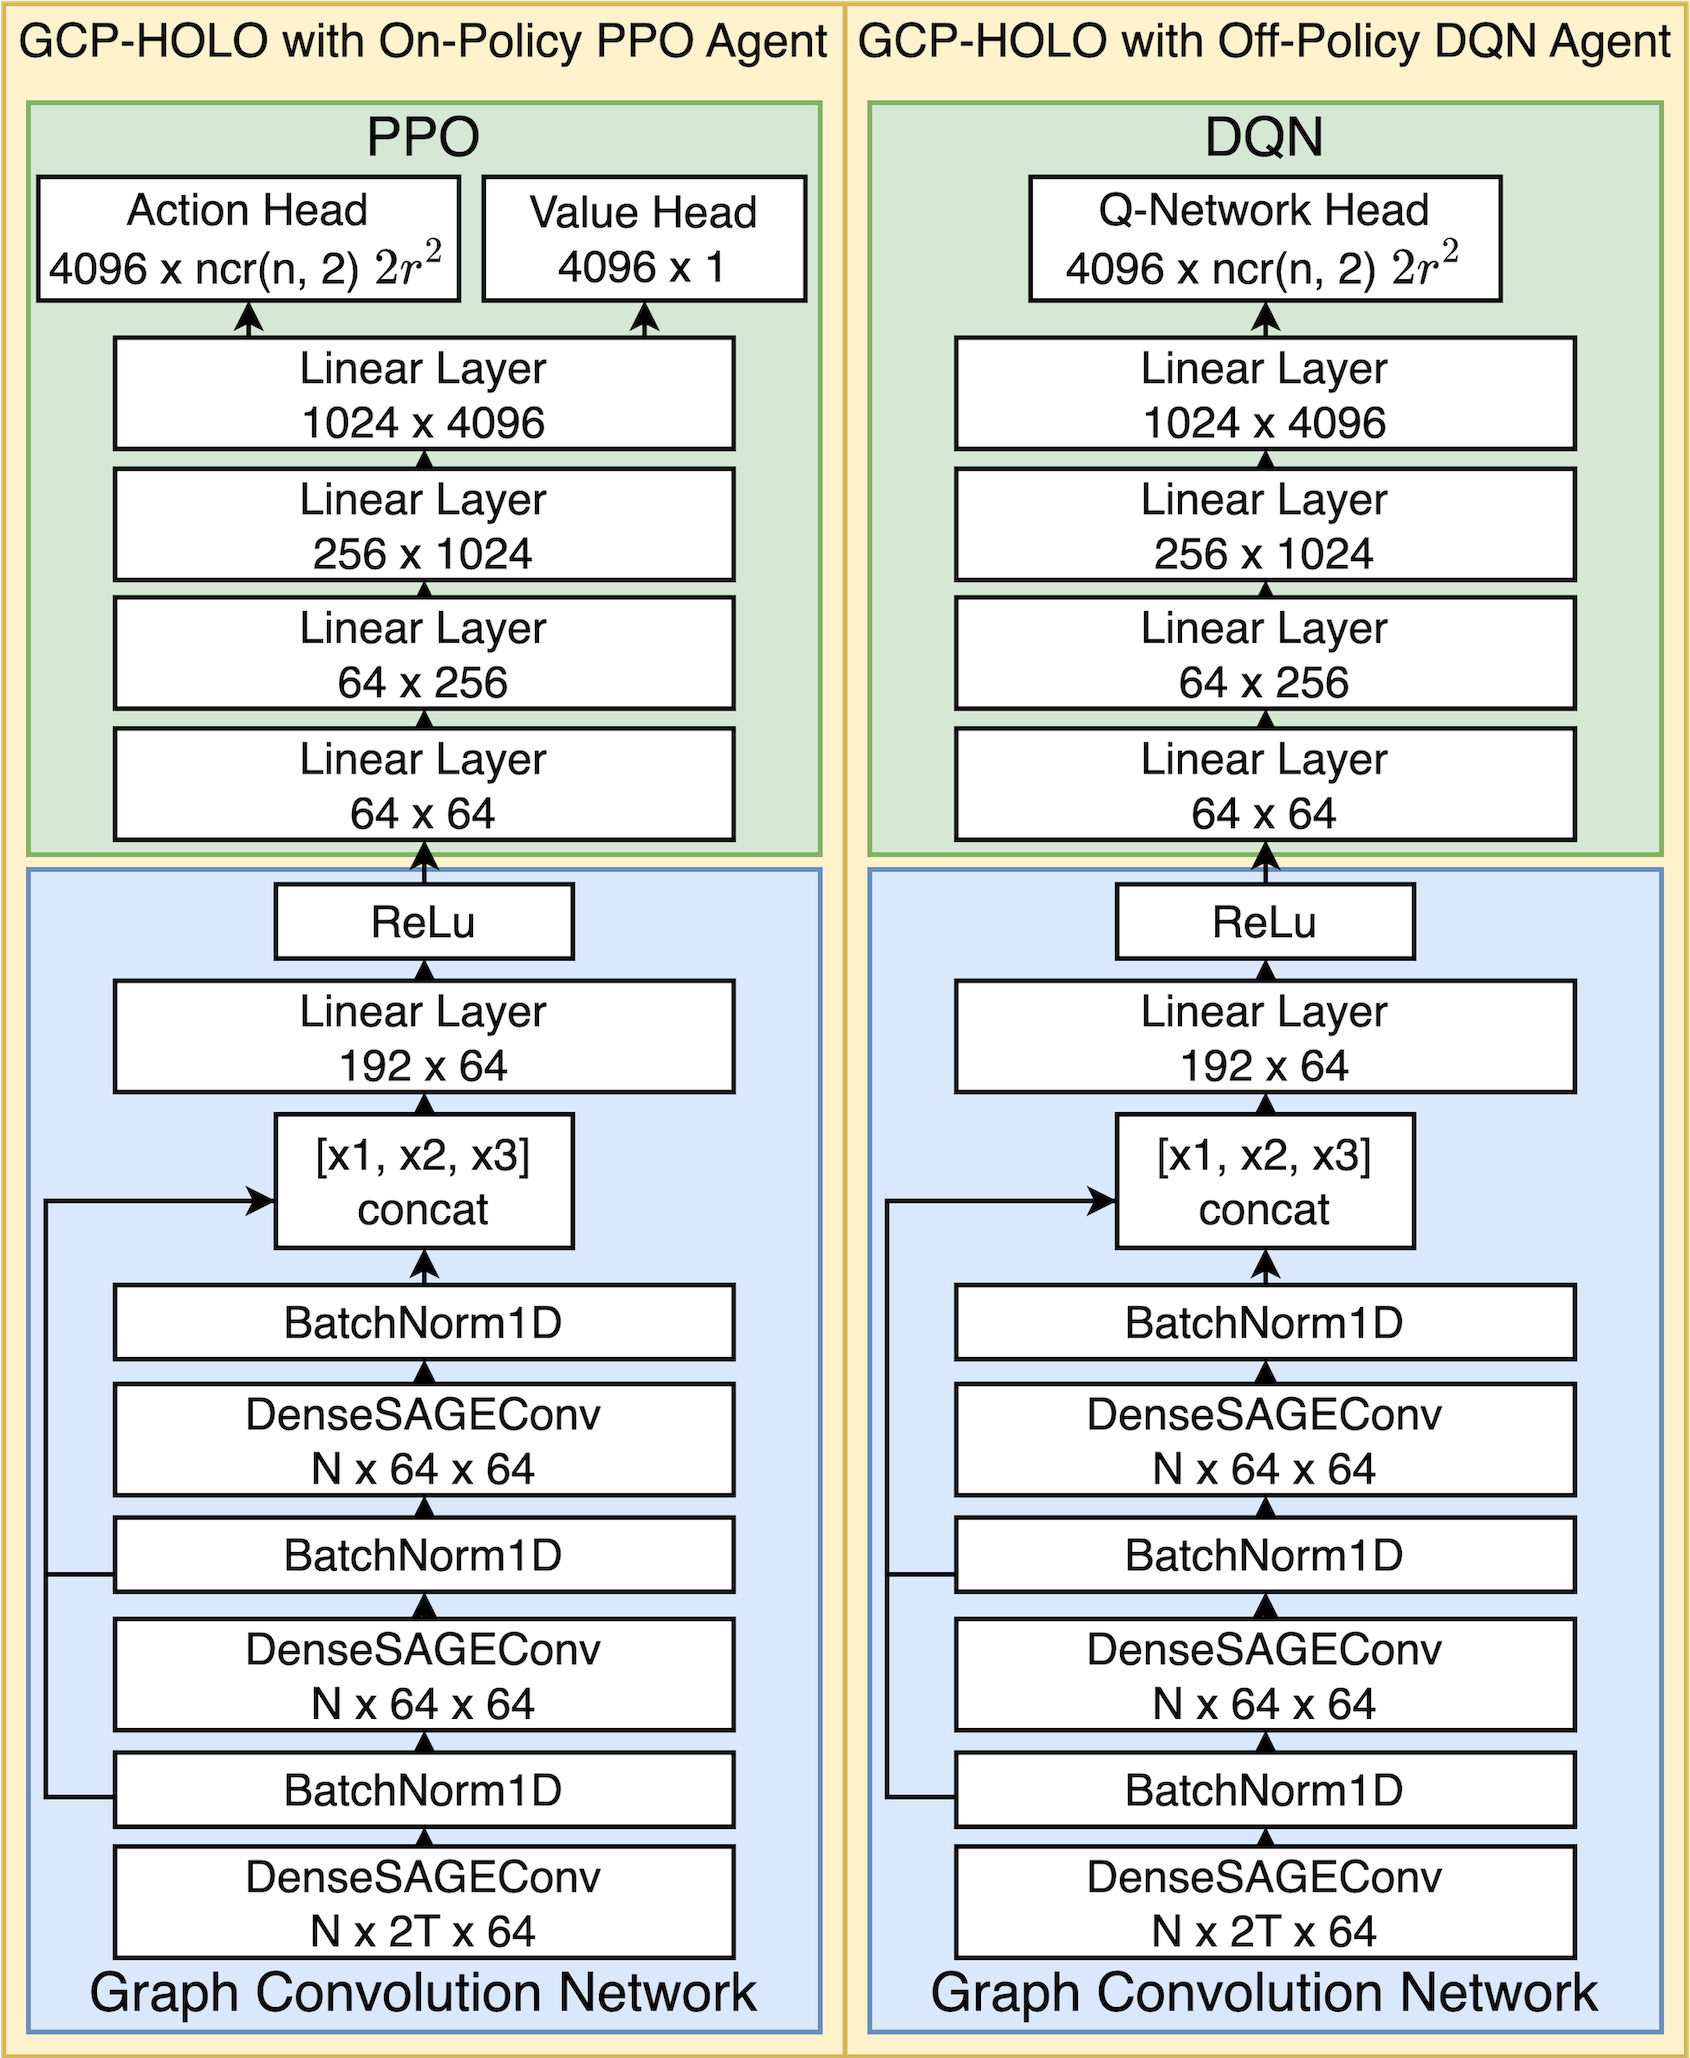
\includegraphics[width=0.7\linewidth]{07_figure_ML_model_architecture.png}
    \caption{GCP-HOLO model architecture with on-policy PPO head or off-policy DQN head}
    \label{fig:ppo-dqn}
\end{figure}

\begin{algorithm}[H]
\caption{Training procedure}
\label{alg:training_procedure}
\begin{algorithmic}[1]
\Require $x'_{\text{goal}},\ \text{res},\ \text{maxNodes},\ \text{bound}$ \Comment{The normalized goal trajectory, resolution, max nodes, and boundary}
\State $bestDesigns \gets \{\}$ \Comment{Initialize best designs as empty dict}
\State $env \gets \textsc{InitializeEnv}(x'_{\text{goal}},\ \text{res},\ \text{maxNodes},\ \text{bound})$ \Comment{Initialize Env}
\State $\theta_{\text{Agent}} \gets \textsc{InitializeAgent}()$ \Comment{Initialize Agent}
\For{training steps $= 1,\ 2,\ \ldots$}
    \State $env.\text{reset}()$ \Comment{Sample initial state from distribution}
    \State $Buffer \gets \textsc{CollectRolloutData}(env,\ \theta_{\text{Agent}})$ \Comment{Collect state, action, reward for training}
    \State $bestDesigns \gets \textsc{UpdateBestDesigns}(Buffer)$ \Comment{Update best designs}
    \If{training step \% update frequency == 0}
        \For{$iter = 1,\ 2,\ \ldots$}
            \State $\theta_{\text{Agent}} \gets \textsc{UpdateAgent}(\theta_{\text{Agent}},\ Buffer)$
        \EndFor
    \EndIf
\EndFor
\State \Return $\theta_{\text{Agent}},\ bestDesigns$
\end{algorithmic}
\end{algorithm}

GCP-HOLO requires the end-user to input the target trajectory, the resolution of the scaffold nodes, the maximum number of nodes, and any design bounds/constraints. The GCP-HOLO algorithm outputs the learned parameters of the neural network models as well as a set of best designs found during training.

\section{Results}\label{sec:gcp:results}
This paper evaluates GCP-HOLO through three experiments. In Sec. \ref{sec:gcp:results:micp}, designs generated by GCP-HOLO on eight test trajectories are compared, with respect to objective value and computation time, to designs generated by Pan et al. \cite{pan_joint_2022}. Section \ref{sec:gcp:results:synthesis} shows an example of a design application with additional body and coupler constraints using GCP-HOLO. Finally, Sec. \ref{sec:gcp:results:policy} provides an ablation study focused on the efficacy of two reinforcement learning algorithm approaches with respect to the breadth of designs and the solution performance. All experiments were run on 1CPU of Intel Xeon Gold 6252 2.10 GHz and used an Nvidia Tesla V100 GPU. The comparative results from Pan et al. were run in that work on a 10-core Intel Xeon(R) W-2155 CPU using all 10-cores \cite{pan_joint_2022}. The hyperparameters used for all experiments are listed in Table \ref{tab:hyper}.

\subsection{GCP-HOLO Versus MICP}\label{sec:gcp:results:micp}
Eight test curves shared by Pan et al. \cite{pan_joint_2022} are used to compare GCP-HOLO performance and their MICP formulation. The objective values of the best designs generated from each of the methods are reported in Fig. \ref{fig:micp-results}. A visual of the designs generated by GCP-HOLO and GCP-HOLO with CMA-ES is shown in Fig. \ref{fig:gcp-results}. For the results shown, GCP-HOLO uses a PPO reinforcement learning agent, trained on 400K steps, which took 35 min. GCP-HOLO sampled 100K designs non-deterministically using the learned policy to generate the solution found; this process took 10 min. The solutions found are at best local minima as GCP-HOLO restricts the initial node location to the discrete scaffold node. To significantly improve the solutions’ performance, an extension that searches other nearby node locations is done using CMA-ES. This extension took less than a minute to converge for each results shown in Figs. \ref{fig:micp-results} and \ref{fig:gcp-results}. 

Figure \ref{fig:micp-results} shows that some solutions generated by GCP-HOLO improve the performance with a 13X speed enhancement over the other approaches. GCP-HOLO found significantly better solutions than all the simulated annealing baselines by Pan et al. on all eight test curves. GCP-HOLO found a better solution from the MICP formulation on two out of the eight test curves with a run time improvement from the reported 10+ h to 45 min. With the extension of CMA-ES global dimensional synthesis, four out of the eight solutions outperform the MICP and mixed integer nonlinear program (MINLP) designs, which Pan et al. reported taking 5–10 h for MINLP to generate or 10+ h for MICP to generate \cite{pan_joint_2022}. The drastic improvement through the global optimization with CMA-ES shows how sensitive the linkage design problem is. The 13X speed improvement seen by GCP-HOLO is in part due to the efficiency of only generating constraint-satisfying linkages and its ability to leverage the GPU. The biggest downside to the MICP method is that before the method converges, the current best design may not be a valid linkage. Pan et al. \cite{pan_joint_2022} show that most of the time of the algorithm is spent trying to find a valid linkage design. In this work, however, by adding the 0DOF linkages to grow the linkage graph with the spatial action constraint, it is easy to generate constraint-satisfying linkages. With the improved efficiency and performance in some instances, GCP-HOLO addresses some of the limitations of Pan et al. \cite{pan_joint_2022} like the linkage generation of high-order linkage graphs and computational complexity.

\begin{figure}
    \centering
    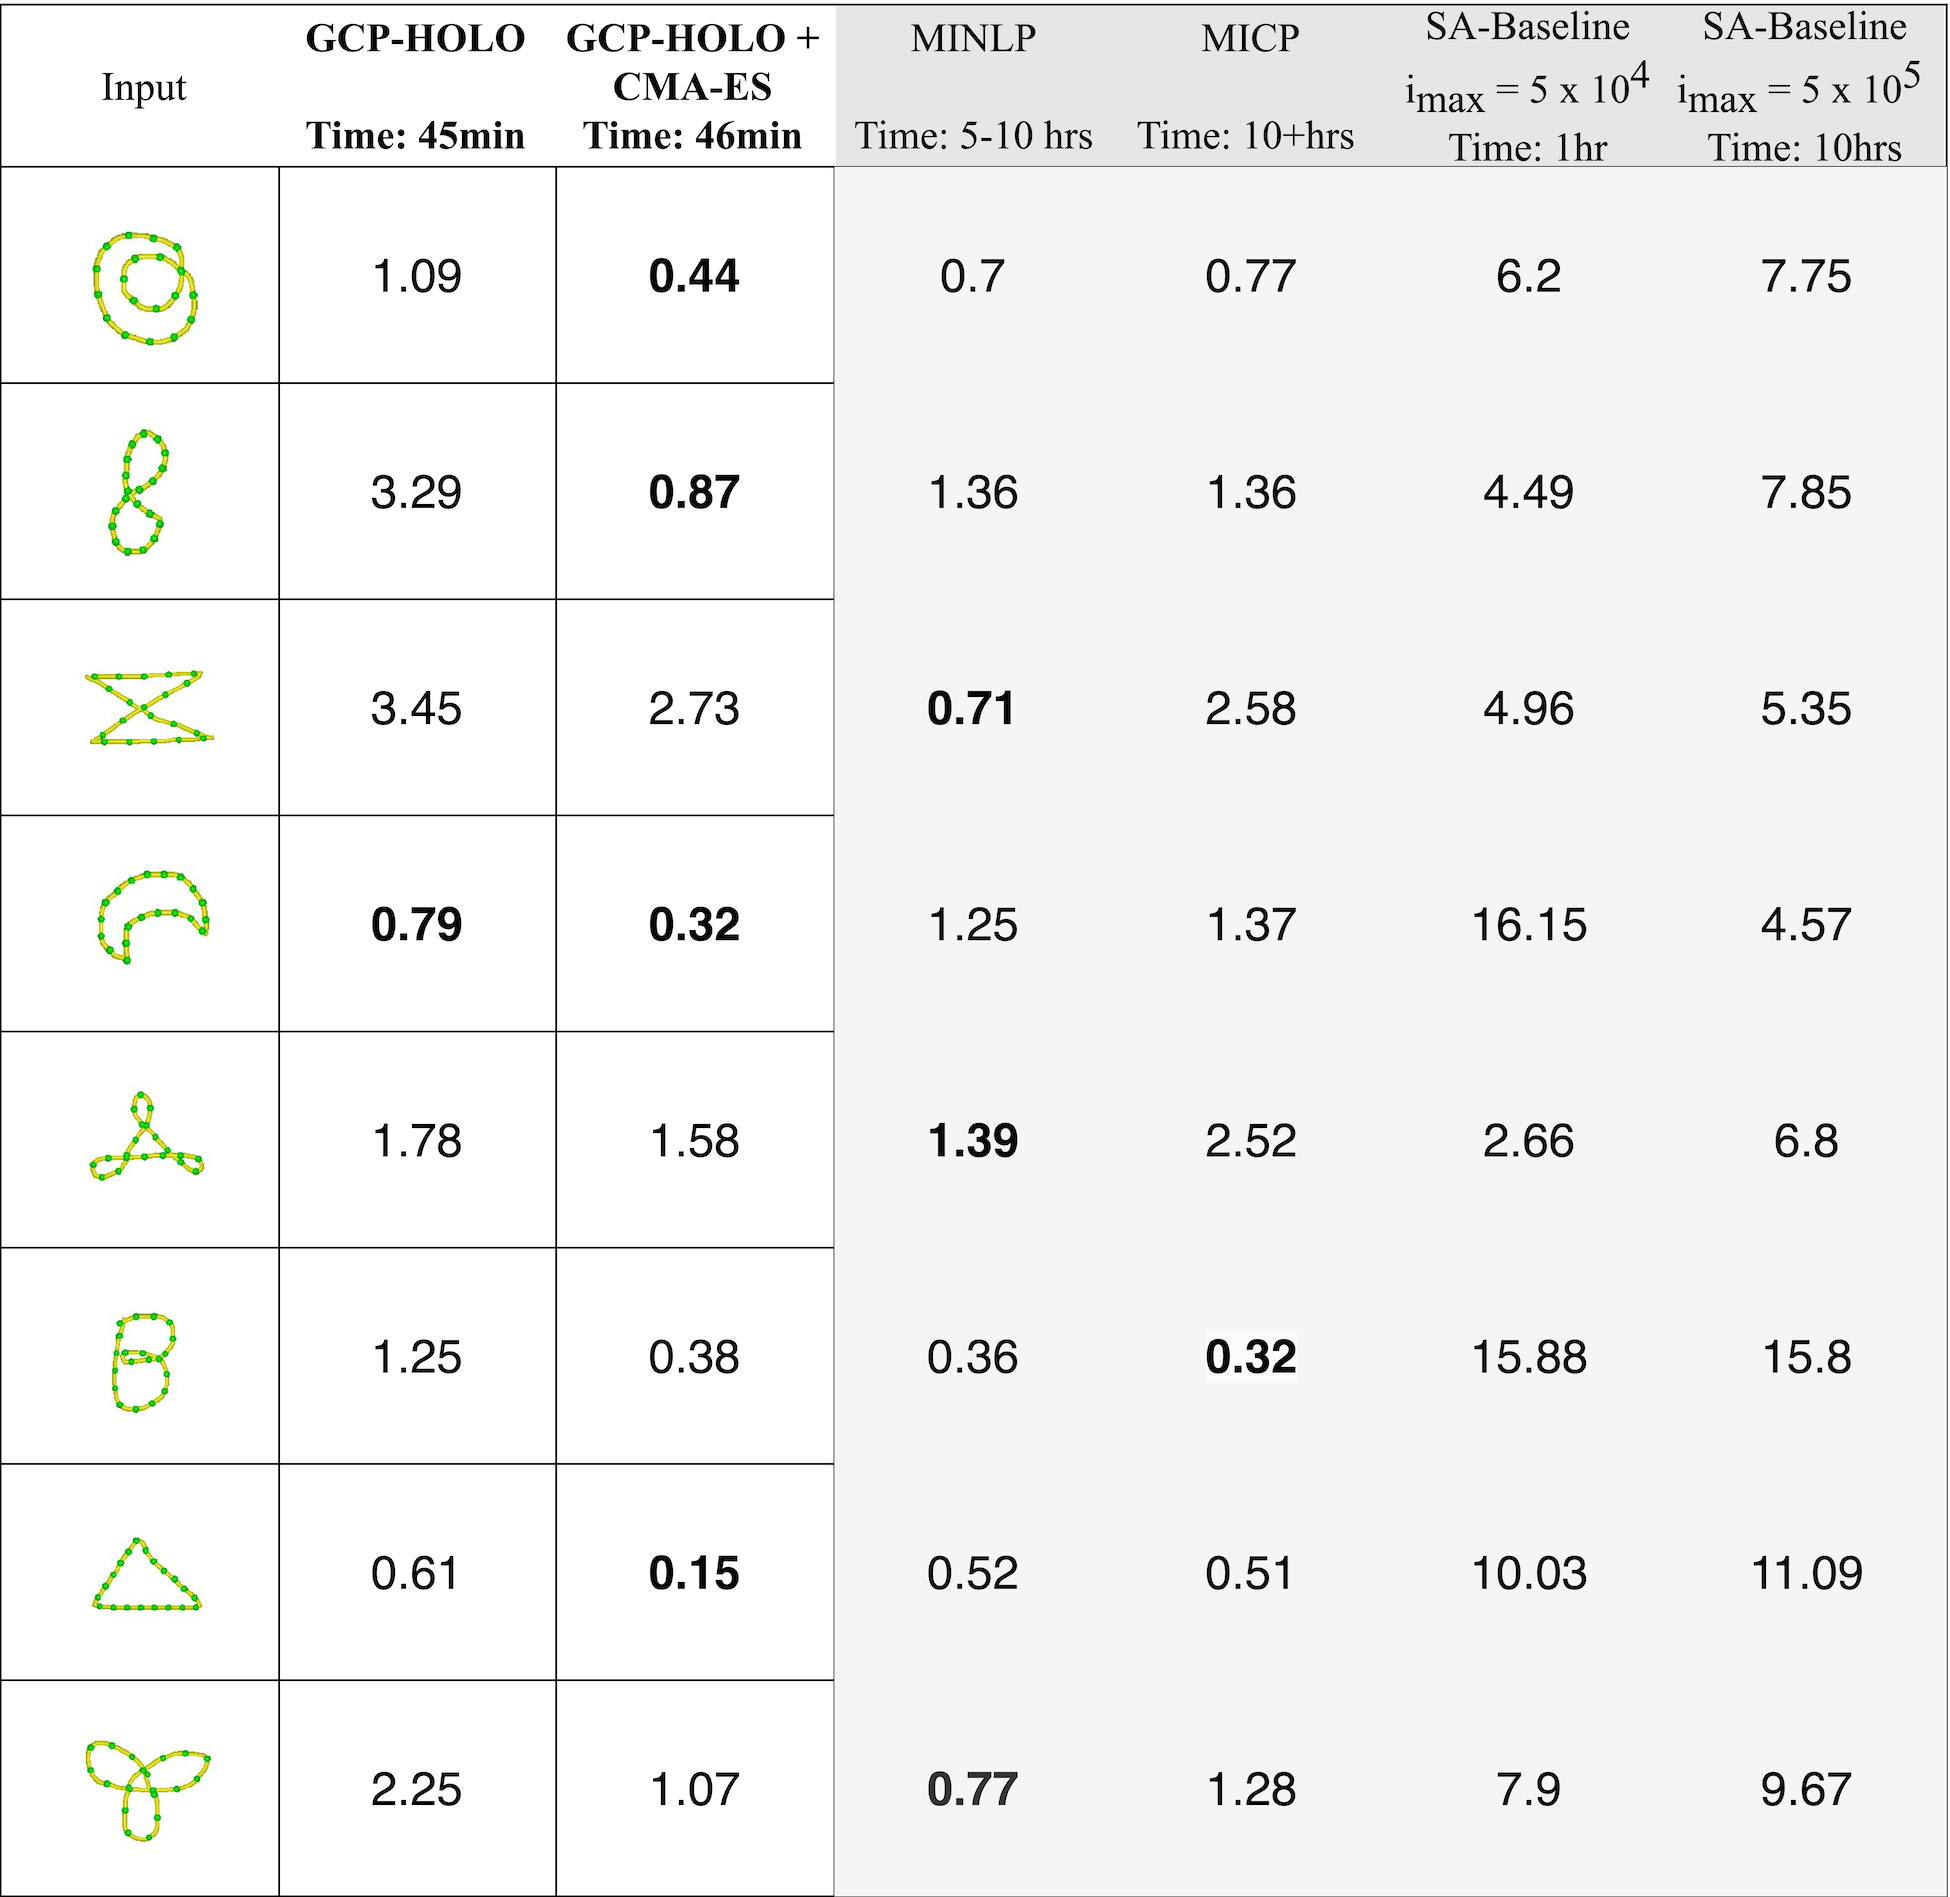
\includegraphics[width=0.9\textwidth]{08_figure_final_comparison_results_simple_table.png}
    \caption{Comparison of best design objective value (lower is better) from GCP-HOLO, GCP-HOLO with CMA-ES on eight test trajectories designed by Pan et al. \cite{pan_joint_2022}. Results from MICP, MINLP, and simulated annealing were taken from Pan et al. \cite{pan_joint_2022}.}
    \label{fig:micp-results}
\end{figure}
\begin{figure}
    \centering
    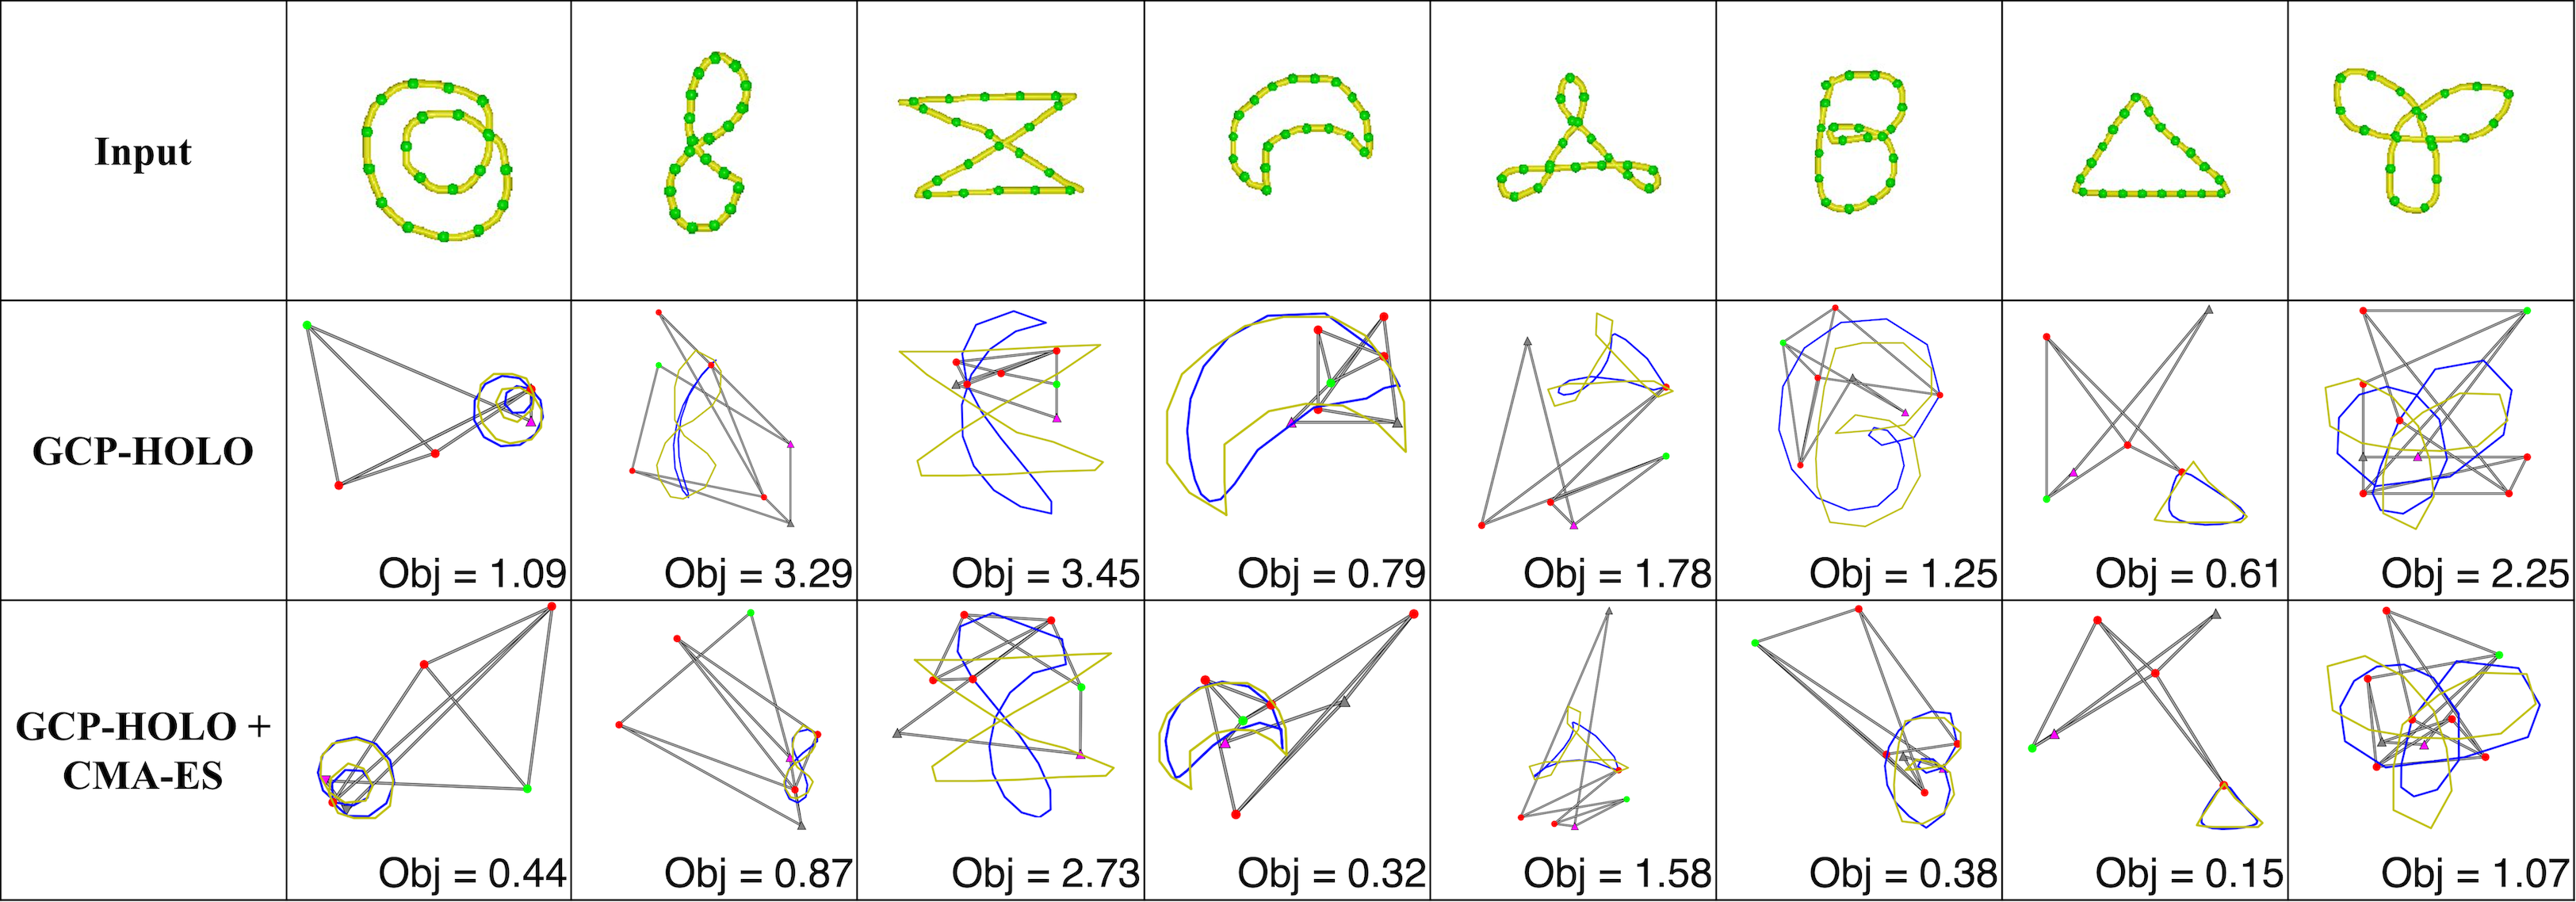
\includegraphics[width=0.9\textwidth]{09_figure_final_comparison_results_01_06.png}
    \caption{Best designs generated from GCP-HOLO, GCP-HOLO with CMA-ES on eight test trajectories designed by Pan et al. \cite{pan_joint_2022}}
    \label{fig:gcp-results}
\end{figure}

\subsection{Path Synthesis Application}\label{sec:gcp:results:synthesis}
In many situations—e.g., designing linkage walking systems, pick and place mechanisms, or construction cranes—it may be necessary to constrain the coupler node in a specific region. In the example here, with results shown in Fig. \ref{fig:constrained-gcp}, an application of designing a walking linkage is shown by generating linkages that satisfy the Trotbot trajectory \cite{Vagle2015TeamTrotbot}. A constraint on the coupler node location in the lower plane and the other node locations in the upper plane was added. The output of GCP-HOLO shows the best designs found for various linkage graph complexities. The solutions generated by GCP-HOLO found designs that minimize the objective and satisfy the constraints with linkage graphs that contain 1–5 cycles. The best design found had three active cycles or an eight-bar linkage.

The top of Fig. \ref{fig:constrained-gcp} shows the solutions generated by an unconstrained GCP-HOLO, which unsurprisingly does not satisfy the constraint condition. The designs generated from the unconstrained GCP-HOLO better minimize the distance to the goal trajectory. In one case, the constrained GCP-HOLO found a better design than the unconstrained GCP-HOLO. One explanation is that the GCP-HOLO method searches the set of designs using only valid actions. Adding the extra constraint of the node locations decreases the number of valid actions, thus decreasing the total number of designs in the search tree. With a smaller search tree, a more significant proportion of designs can be explored, and better solutions found.

\begin{figure}
    \centering
    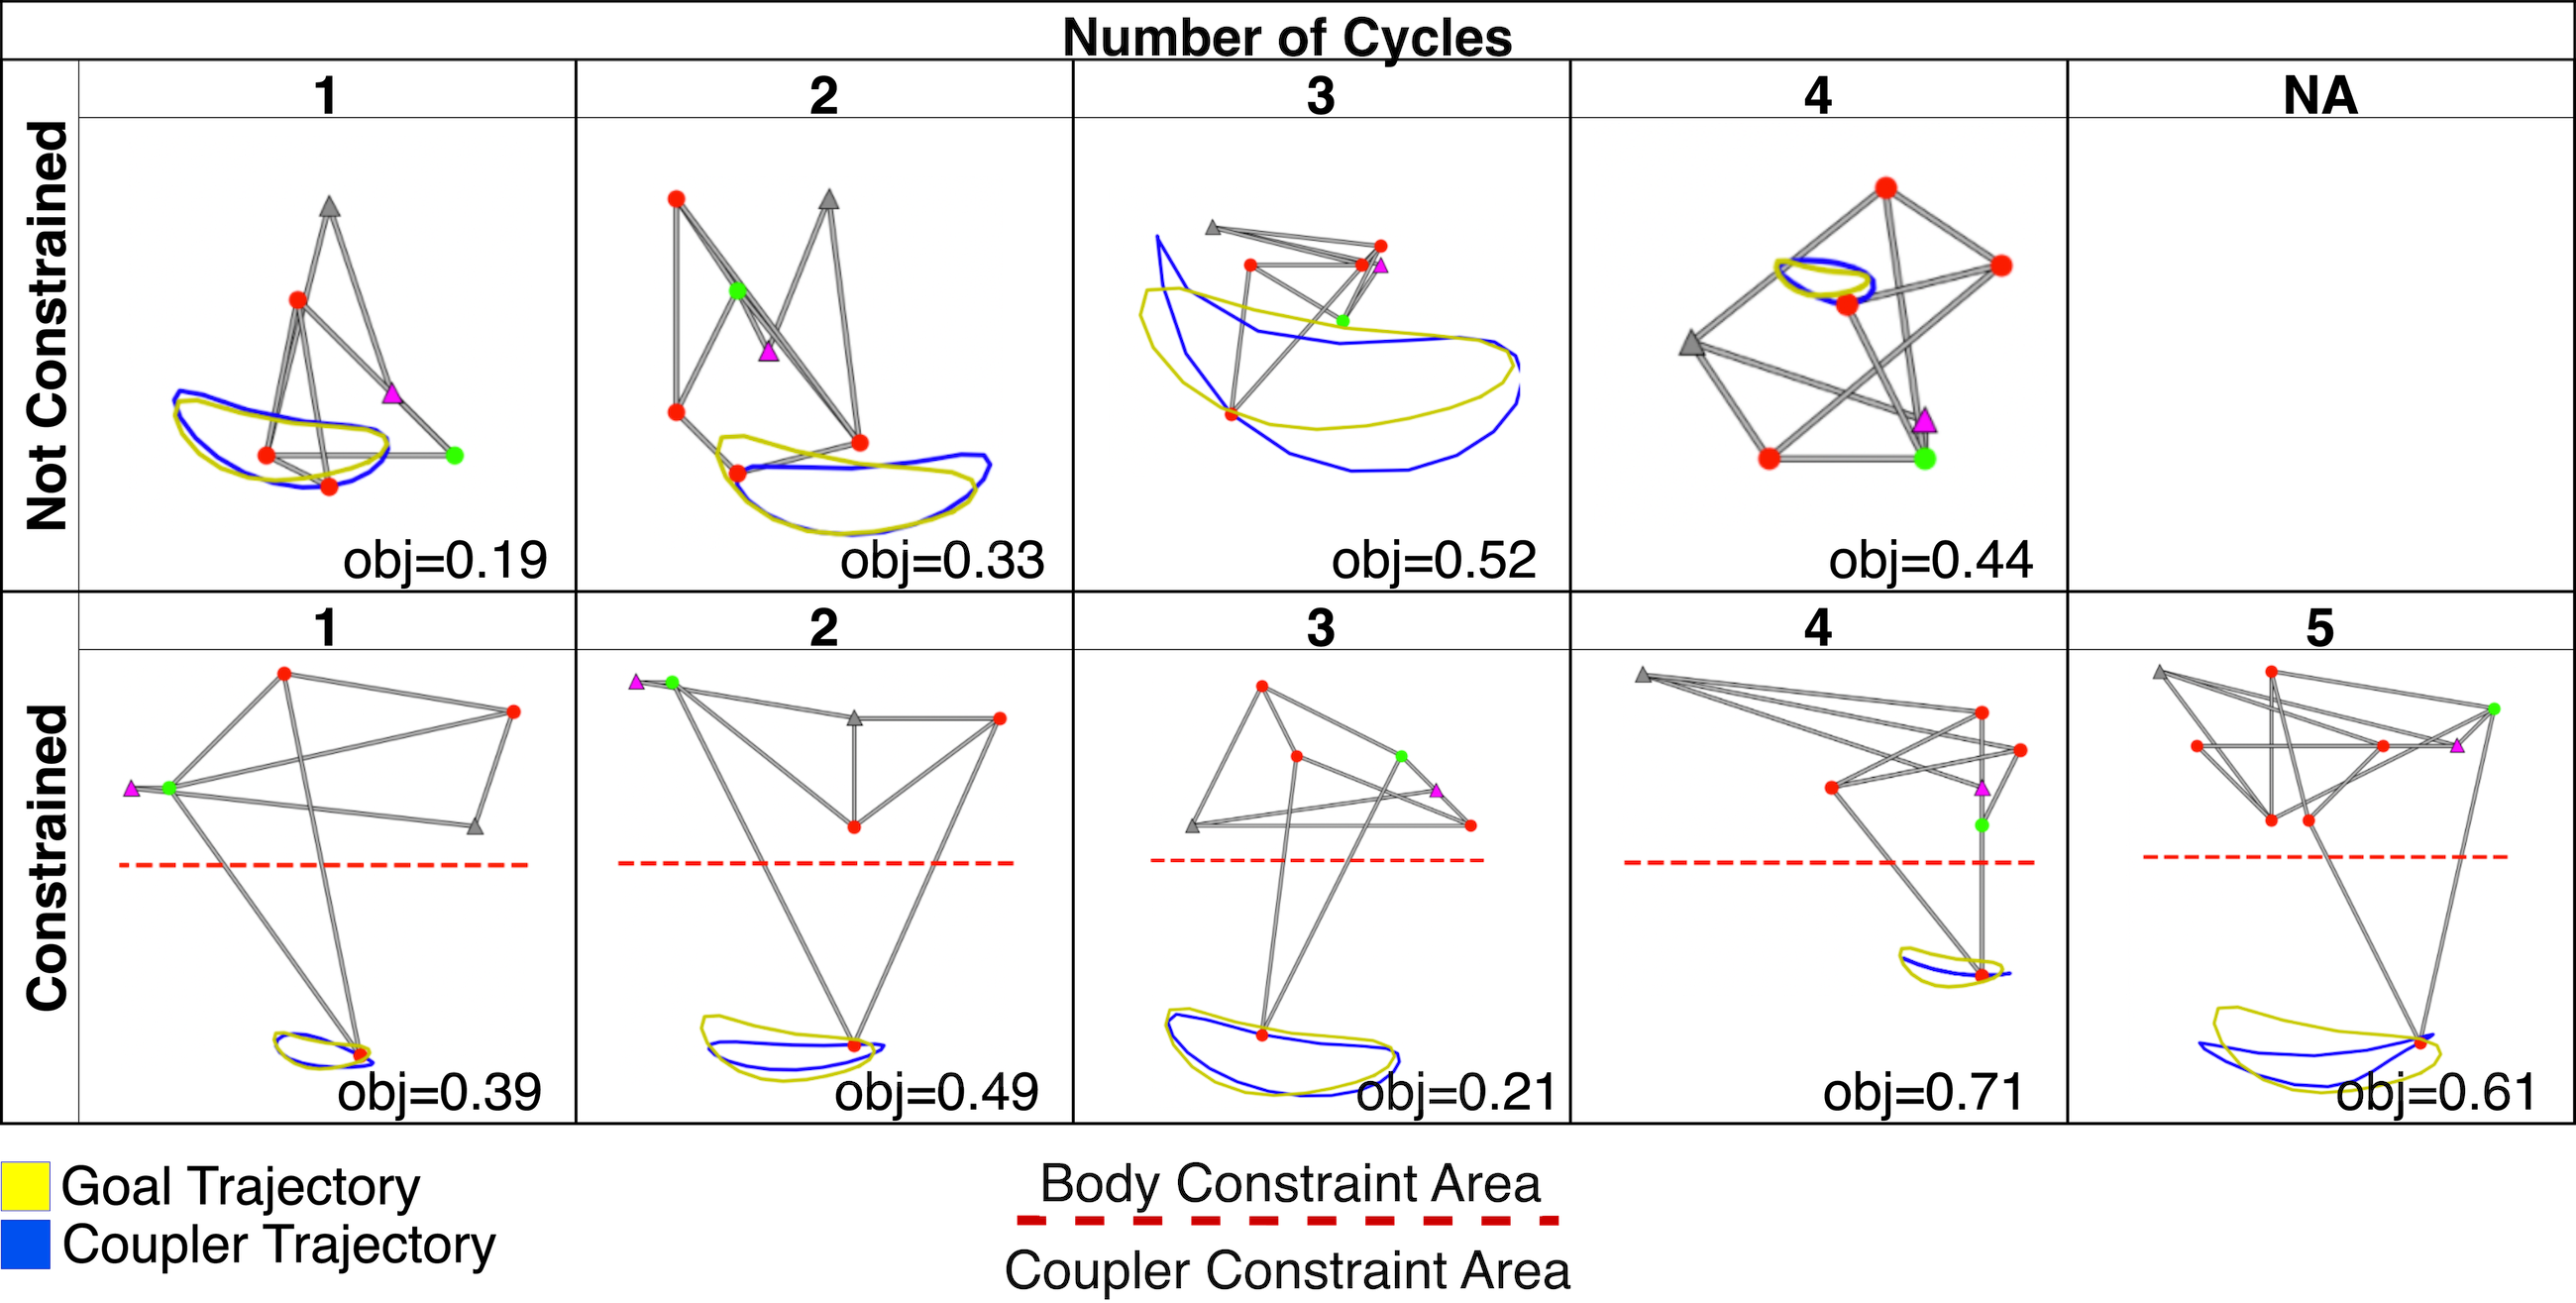
\includegraphics[width=0.9\linewidth]{10_figure_Constraint_example.png}
    \caption{Designs generated by unconstrained GCP-HOLO and constrained GCP-HOLO with TrotBot goal trajectory}
    \label{fig:constrained-gcp}
\end{figure}

\begin{table}[ht]
\centering
\caption{Hyperparameters for GCP-HOLO used in all experiments}\label{tab:hyper}
\resizebox{\textwidth}{!}{
\begin{tabular}{cccccccccc}
\toprule
\parbox{2cm}{\centering Max\\nodes} 
& \parbox{2cm}{\centering Scaffold\\resolution} 
& \parbox{2cm}{\centering Trajectory\\samples} 
& \parbox{2cm}{\centering Learning\\rate} 
& \parbox{2cm}{\centering Batch\\size} 
& \parbox{2cm}{\centering Number\\envs} 
& \parbox{2cm}{\centering Training\\steps} 
& \parbox{2cm}{\centering Eval\\episodes} 
& \parbox{2cm}{\centering Sigma\\CMA-ES} 
& \parbox{2cm}{\centering Tol\\CMA-ES} \\
\midrule
11 & 11 & 20 & \(1 \times 10^{-4}\) & \(1 \times 10^4\) & 100 & \(4 \times 10^5\) & \(1 \times 10^5\) & \(5 \times 10^{-5}\) & \(1 \times 10^{-4}\) \\
\bottomrule
\end{tabular}
}
\end{table}

\subsection{On-Versus Off-Policy Comparison}\label{sec:gcp:results:policy}
Any policy can generate a variety of linkages using the GCP-HOLO action space, but the breadth of solutions that span various linkage topologies may be limited. Designs that span different linkage graph topologies enable better starting points for further exploration and assessment. In this ablation study, a trained GCP-HOLO model with an on-policy PPO policy, a trained GCP-HOLO model with an off-policy DQN policy, and a random search each generate 20 trials of 100K linkage designs. All policies are trained with the Jansen linkage trajectory set as the goal \cite{Jansen1990Strandbeast}. The designs generated are pruned and separated into groups based on the number of active cycles that comprise the linkage graph. The distributions of the designs are evaluated on the number of high-order linkage graphs that were generated and given in Table \ref{tab:gcp:2}, the minimum distance measured (the best design) presented in Table \ref{tab:gcp:3}, the mean distance measured given in Table \ref{tab:gcp:4}, and the number of invalid linkages generated and shown in Fig. \ref{fig:ppo-invalid}. The average over the 20 trials and the standard error are presented in each table. Table \ref{tab:gcp:2} shows that GCP-HOLO with PPO generates the most high-order linkage graphs. In some high-order linkage graphs, GCP-HOLO with DQN generates more designs; this is not unexpected as the policies are stochastic. By generating more high-order linkage graphs, it is more likely that GCP-HOLO will find better designs for minimizing the distance to the goal. PPO found significant improvement in the average best design generated over the other approaches in five of the six high-order linkage graph types. In Table~\ref{tab:gcp:3}, these designs represent the ones with the best performance with respect to the objective function. This shows that the PPO agent is more likely to find designs that better satisfy the primary objective. Table~\ref{tab:gcp:4} shows the average performance of all designs generated by the various approaches. Table~\ref{tab:gcp:4} excludes values reported for instances where less than ten designs are generated because the statistical methods are not indicative of distribution. Table~\ref{tab:gcp:4} shows that, on average, the designs generated by GCP-HOLO with PPO agent were better than other approaches.These distributions are important to consider since there may be objectives that are not explicit in the optimization, such as manufacturability and aesthetics. Generating sets of designs improves the end-user selections. Finally, Fig.~\ref{fig:ppo-invalid} shows that the PPO agent generated the fewest number of invalid designs. While the scaffold node simplified constraint satisfaction criteria shown in Algorithm~\ref{alg:valid_scaffold} reduces the number of invalid actions, it does not prevent them altogether. Both DQN and PPO reduce the number of invalid designs generated, but PPO far reduces that number in comparison to the other approaches. 

\begin{figure}
    \centering
    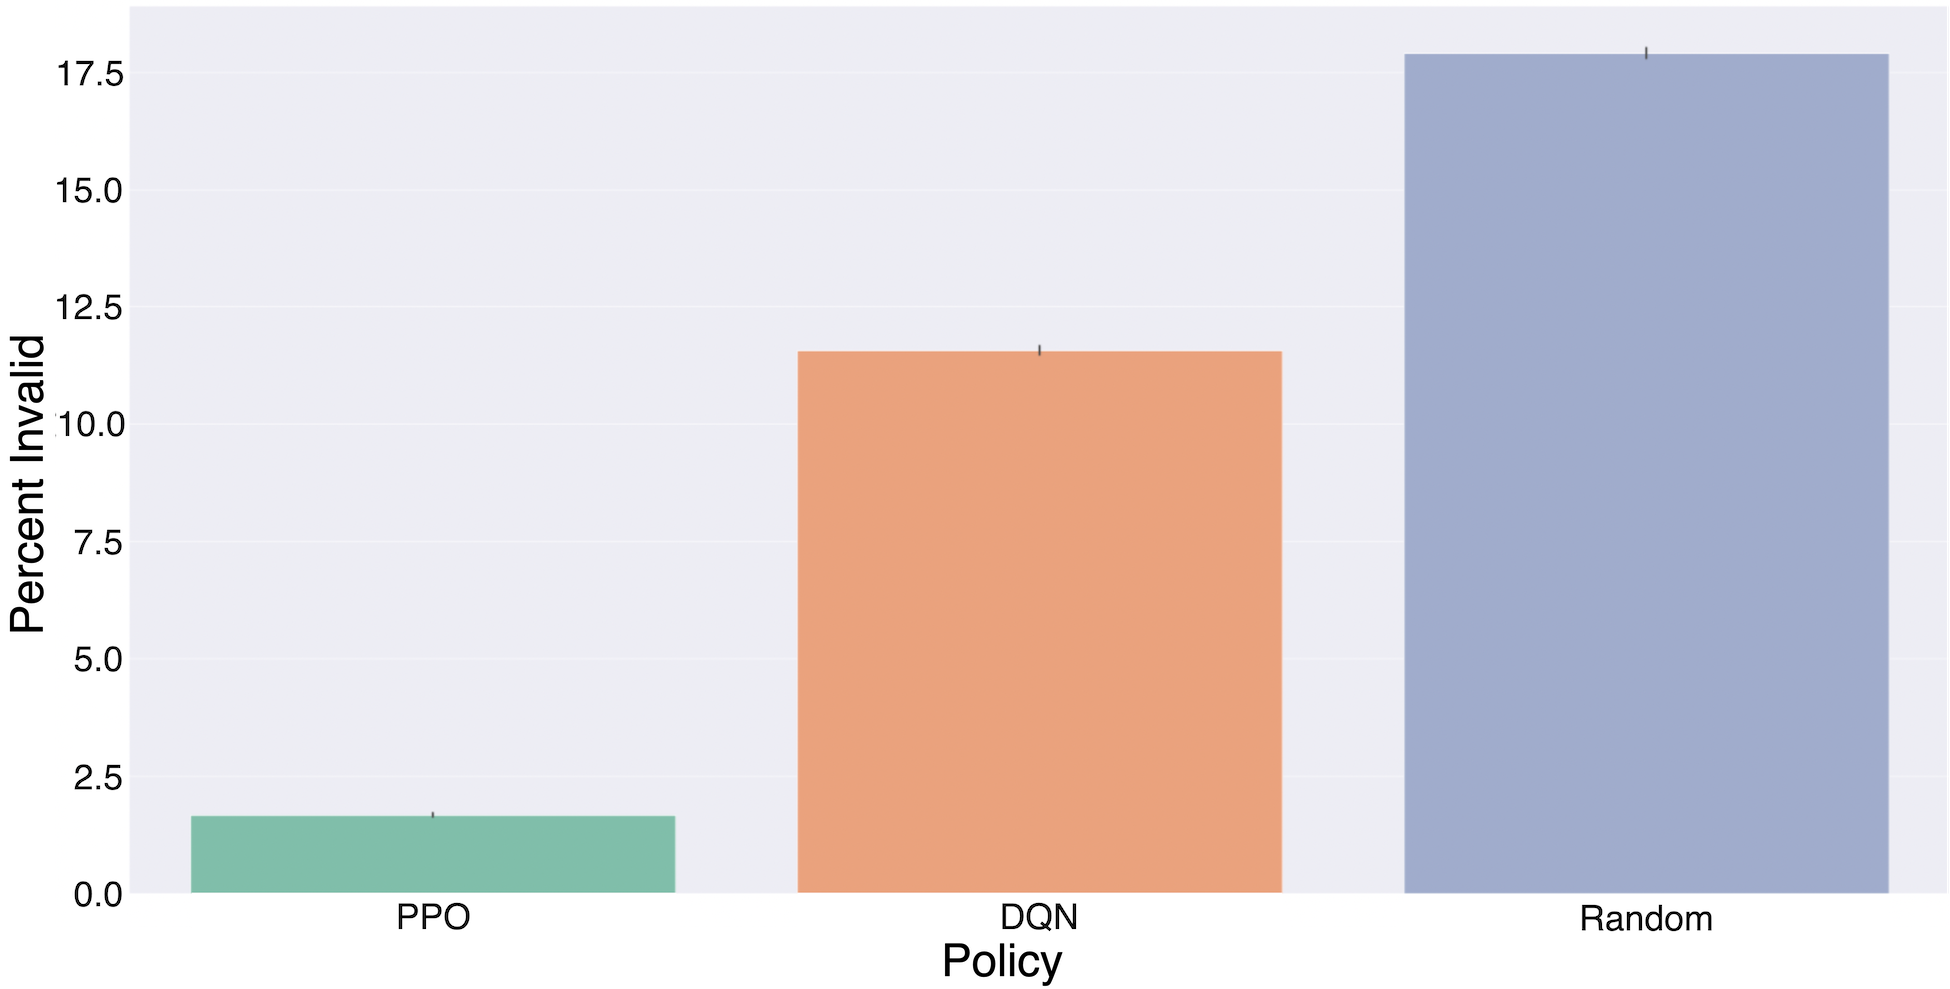
\includegraphics[width=\linewidth]{11_figure_percent_invalid.png}
    \caption{Average number of invalid designs generated for each policy}
    \label{fig:ppo-invalid}
\end{figure}

This comparison between the GCP-HOLO model with PPO policy, the GCP-HOLO model with DQN policy, and random search shows that the learned search heuristic from both PPO and DQN generates better designs than random search. It also presents several advantages of the PPO policy over the DQN policy, such as the breadth of designs and performance of solutions. For these reasons, using GCP-HOLO with the PPO policy is recommended.

\begin{table}[h]
\centering
\caption{Comparison of GCP-HOLO with on-policy PPO policy, GCP-HOLO with off-policy DQN policy, and random policy on the number of designs generated in various linkage graph topologies}\label{tab:gcp:2}
\resizebox{\textwidth}{!}{
\begin{tabular}{lcccccccc}
\toprule
\textbf{Cycles} & \textbf{1} & \textbf{2} & \textbf{3} & \textbf{4} & \textbf{5} & \textbf{6} & \textbf{7} & \textbf{8} \\
\midrule
PPO & $27{,}343 \pm 131$ & $28{,}541 \pm 127$ & $\mathbf{28{,}466 \pm 107}^\text{a}$ & $\mathbf{11{,}133 \pm 89}^\text{a}$ & $\mathbf{2445 \pm 45}^\text{a}$ & $375 \pm 20$ & $20 \pm 4$ & $1 \pm 0.7$ \\
DQN & $23{,}509 \pm 225$ & $\mathbf{32{,}884 \pm 197}^\text{a}$ & $21{,}005 \pm 149$ & $8511 \pm 87$ & $1920 \pm 39$ & $\mathbf{560 \pm 28}^\text{a}$ & $\mathbf{31 \pm 5}^\text{a}$ & $1 \pm 0.6$ \\
Random & $\mathbf{29{,}886 \pm 129}^\text{a}$ & $32{,}171 \pm 186$ & $15{,}251 \pm 83$ & $4002 \pm 52$ & $675 \pm 23$ & $95 \pm 8$ & $7 \pm 2$ & $0 \pm 0.5$ \\
\bottomrule
\end{tabular}
}
\begin{flushleft}
\footnotesize{$^\text{a}$Statistically significant.}
\end{flushleft}
\end{table}

\begin{table}[h]
\centering
\caption{Comparison of GCP-HOLO with on-policy PPO policy, GCP-HOLO with off-policy DQN policy, and random policy on the minimum error of designs generated in various linkage graph topologies}\label{tab:gcp:3}
\resizebox{\textwidth}{!}{
\begin{tabular}{lcccccccc}
\toprule
\textbf{Cycles} & \textbf{1} & \textbf{2} & \textbf{3} & \textbf{4} & \textbf{5} & \textbf{6} & \textbf{7} & \textbf{8} \\
\midrule
PPO & $0.44 \pm 0.007$ & $0.43 \pm 0.011$ & $\mathbf{0.28 \pm 0.014}$ & $0.38 \pm 0.014$ & $\mathbf{0.47 \pm 0.015}^\text{a}$ & $\mathbf{0.62 \pm 0.029}^\text{a}$ & $1.63 \pm 0.180$ & $\mathbf{5.15 \pm 0.63}^\text{a}$ \\
DQN & $\mathbf{0.35 \pm 0.005}^\text{a}$ & $\mathbf{0.34 \pm 0.007}^\text{a}$ & $0.27 \pm 0.009$ & $0.39 \pm 0.017$ & $0.54 \pm 0.031$ & $0.68 \pm 0.057$ & $\mathbf{1.60 \pm 0.167}$ & $7.33 \pm 2.52$ \\
Random & $0.38 \pm 0.011$ & $0.38 \pm 0.016$ & $0.32 \pm 0.014$ & $0.44 \pm 0.017$ & $0.61 \pm 0.027$ & $0.99 \pm 0.077$ & $2.822 \pm 0.29$ & $7.62 \pm 3.15$ \\
\bottomrule
\end{tabular}
}
\begin{flushleft}
\footnotesize{$^\text{a}$Statistically significant.}
\end{flushleft}
\end{table}

\begin{table}[h]
\centering
\caption{Comparison of GCP-HOLO with on-policy PPO policy, GCP-HOLO with off-policy DQN policy, and random policy on the average error of designs generated in various linkage graph topologies}\label{tab:gcp:4}
\resizebox{\textwidth}{!}{
\begin{tabular}{lcccccccc}
\toprule
\textbf{Cycles} & \textbf{1} & \textbf{2} & \textbf{3} & \textbf{4} & \textbf{5} & \textbf{6} & \textbf{7} & \textbf{8} \\
\midrule
PPO & $7.1 \pm 0.01$ & $\mathbf{7.1 \pm 0.01}^\text{a}$ & $\mathbf{6.8 \pm 0.01}^\text{a}$ & $\mathbf{7.4 \pm 0.01}^\text{a}$ & $\mathbf{7.5 \pm 0.03}^\text{a}$ & $\mathbf{7.8 \pm 0.07}^\text{a}$ & $8.4 \pm 0.41$ & --- \\
DQN & $7.1 \pm 0.01$ & $8.7 \pm 0.01$ & $7.5 \pm 0.01$ & $8.5 \pm 0.02$ & $8.8 \pm 0.03$ & $8.6 \pm 0.04$ & $\mathbf{7.1 \pm 0.25}$ & --- \\
Random & $7.1 \pm 0.01$ & $8.0 \pm 0.01$ & $7.8 \pm 0.01$ & $7.9 \pm 0.02$ & $7.9 \pm 0.05$ & $8.2 \pm 0.015$ & --- & --- \\
\bottomrule
\end{tabular}
}
\begin{flushleft}
\footnotesize{$^\text{a}$Statistically significant.}
\end{flushleft}
\end{table}

\section{Discussion}
GCP-HOLO uses a learned stochastic search approach for generating constraint satisfying high-order linkage graphs for the inverse design of linkages. Section~\ref{sec:gcp:results:micp} shows that the solutions generated by GCP-HOLO achieved a lower target trajectory distance value on 25\% of the test trajectories compared to the MICP formulation while reducing the computational complexity by 13X. The solutions outperform the state-of-the-art method in 50\% of the test cases when using the generated designs as initial positions for further optimization using CMA-ES. Section~\ref{sec:gcp:results:synthesis} shows an application of GCP-HOLO with additional constraints, generating designs with varying linkage graph complexity. The breadth of design solutions can be a starting point to explore further by the end-user, such as evaluating aesthetics or manufacturability. Section~\ref{sec:gcp:results:policy} characterizes two reinforcement learning policies that can be used in GCP-HOLO for this problem. Section~\ref{sec:gcp:results:policy} demonstrates that PPO generates significantly more high-order linkage designs, generates the designs with the best performance, improves design distribution performance, and reduces the number of invalid designs susceptible to this method.

While GCP-HOLO presents improvements to the complex path synthesis problem for generating linkages that satisfy the desired kinematic behavior, several limitations still exist. First, since GCP-HOLO is a stochastic search algorithm, there are no guarantees this paper can make about optimality in a finite time horizon, but similar methods have been shown to generate optimally directed solutions in multi-modal discontinuous problems \cite{you_graph_2018, zhao_robogrammar_2020}. Next, the dimensionality of the linkages generated should be able to satisfy the path synthesis problem better. Still, the current discrete action space strongly limits the performance of the method due to the sensitivity of the dimensional synthesis problem. One approach could be to extend GCP-HOLO through a bi-level process where GCP-HOLO proposes constraint satisfying initial states and secondary optimization methods further improve the solution. Another interesting extension would be to incorporate relaxations to the discretization of the design spaces shown in Raina et al. \cite{raina_design_2021}, to generate new node locations that are not confined to the scaffold node grid. The topological rule used in this work cannot generate all topological variants; understanding which topologies are suited for the desired path and finding new topological rules to span all linkage topologies is an interesting direction. Another key limitation is the lack of manufacturability considerations when generating linkages with GCP-HOLO. To further support non-experts in designing linkages, manufacturability, link conflicts, stresses, and end effector dynamics must be considered. GCP-HOLO currently only supports 1DOF planar linkage design, but spatial linkage design could be considered using a similar generation technique. The hardest challenge is that the action space becomes proportional to $r^3$, greatly increasing the branching factor. However, adding 0DOF spatial linkages to grow the linkage graph with scaffold nodes iteratively would enable the design of linkages outside the plane.

\section{Conclusion}
GCP-HOLO is an RL-based tree search method that leverages a graph expansion rule and recursive kinematics to efficiently search for high-order linkage graphs that satisfy the path synthesis problem. Compared to other state-of-the-art methods, GCP-HOLO performs 13X faster. GCP-HOLO learns a stochastic search policy to find solutions by exploring the tree of valid linkages. The solutions generated by GCP-HOLO can be extended with geometric optimization of the node positions, which results in designs that perform the best on 50\% of the test cases. This paper shows an application of designing a linkage for a walking system using GCP-HOLO that satisfies additional constraints related to the body and coupler positions. GCP-HOLO is a general method for path synthesis which has applications in many areas from automotive, space, and construction, where linkages play a role in their systems. This paper showed that PPO, an on-policy agent, was advantageous to DQN, an off-policy agent, for this problem. This paper presents a method that reduces the end user’s domain expertise needed by generating sets of solutions of varying linkage graph complexity, extending the capabilities of design systems and mechanical designers in creating future design solutions.

%%% Local Variables:
%%% coding: utf-8
%%% mode: latex
%%% TeX-engine: xetex
%%% TeX-master: "../thesis"
%%% End: